\PassOptionsToPackage{usenames, dvipsnames}{xcolor}
%% For double-blind review submission, w/o CCS and ACM Reference (max submission space)
% \documentclass[sigplan,10pt,review,anonymous]{acmart}\settopmatter{printfolios=true,printccs=false,printacmref=false}
%% For double-blind review submission, w/ CCS and ACM Reference
%\documentclass[sigplan,10pt,review,anonymous]{acmart}\settopmatter{printfolios=true}
%% For single-blind review submission, w/o CCS and ACM Reference (max submission space)
\documentclass[sigplan,9pt,review]{acmart}\settopmatter{printfolios=true,printccs=false,printacmref=false}
%% For single-blind review submission, w/ CCS and ACM Reference
%\documentclass[sigplan,10pt,review]{acmart}\settopmatter{printfolios=true}
%% For final camera-ready submission, w/ required CCS and ACM Reference
%\documentclass[sigplan,10pt]{acmart}\settopmatter{}


%% Conference information
%% Supplied to authors by publisher for camera-ready submission;
%% use defaults for review submission.
\acmConference[PL'18]{ACM SIGPLAN Haskell Symposium}{September 27--28, 2018}{St. Louis, MO, USA}
\acmYear{2018}
\acmISBN{} % \acmISBN{978-x-xxxx-xxxx-x/YY/MM}
\acmDOI{} % \acmDOI{10.1145/nnnnnnn.nnnnnnn}
\startPage{1}

%% Copyright information
%% Supplied to authors (based on authors' rights management selection;
%% see authors.acm.org) by publisher for camera-ready submission;
%% use 'none' for review submission.
\setcopyright{none}
%\setcopyright{acmcopyright}
%\setcopyright{acmlicensed}
%\setcopyright{rightsretained}
%\copyrightyear{2017}           %% If different from \acmYear

%% Bibliography style
\bibliographystyle{ACM-Reference-Format}
%% Citation style
%\citestyle{acmauthoryear}  %% For author/year citations
%\citestyle{acmnumeric}     %% For numeric citations
%\setcitestyle{nosort}      %% With 'acmnumeric', to disable automatic
                            %% sorting of references within a single citation;
                            %% e.g., \cite{Smith99,Carpenter05,Baker12}
                            %% rendered as [14,5,2] rather than [2,5,14].
%\setcitesyle{nocompress}   %% With 'acmnumeric', to disable automatic
                            %% compression of sequential references within a
                            %% single citation;
                            %% e.g., \cite{Baker12,Baker14,Baker16}
                            %% rendered as [2,3,4] rather than [2-4].


%%%%%%%%%%%%%%%%%%%%%%%%%%%%%%%%%%%%%%%%%%%%%%%%%%%%%%%%%%%%%%%%%%%%%%
%% Note: Authors migrating a paper from traditional SIGPLAN
%% proceedings format to PACMPL format must update the
%% '\documentclass' and topmatter commands above; see
%% 'acmart-pacmpl-template.tex'.
%%%%%%%%%%%%%%%%%%%%%%%%%%%%%%%%%%%%%%%%%%%%%%%%%%%%%%%%%%%%%%%%%%%%%%


%% Some recommended packages.
\usepackage{booktabs}   %% For formal tables:
                        %% http://ctan.org/pkg/booktabs
\usepackage{subcaption} %% For complex figures with subfigures/subcaptions
                        %% http://ctan.org/pkg/subcaption
\usepackage{unicode-math}
\usepackage{xspace}
\usepackage{xparse}
\usepackage{minted}
\usepackage{mathpartir}
\usepackage{placeins}
\usepackage{relsize}
\usepackage{chngcntr}
\usepackage{float}
\usepackage{hyperref}
\usepackage[title]{appendix}

\setmathsf{Linux Biolinum}
\setminted{fontsize=\small}

\newcommand{\clott}{\textsf{CloTT}\xspace}
\newcommand{\clopl}{\textsf{CloPL}\xspace}
\newcommand{\code}[1]{\texttt{#1}}


\usepackage{amsmath,amsfonts,amsthm,stmaryrd}

\usepackage{xspace}
\usepackage{MnSymbol}
\usepackage[shortlabels,inline]{enumitem}

% \theoremstyle{definition}\newtheorem{definition}{Definition}[section]
% \newtheorem{theorem}[definition]{Theorem}
% \theoremstyle{theorem}\newtheorem{axiom}[definition]{Axiom}
% \theoremstyle{theorem}\newtheorem{lemma}[definition]{Lemma}
% \theoremstyle{theorem}\newtheorem{proposition}[definition]{Proposition}
% \theoremstyle{theorem}\newtheorem{corollary}[definition]{Corollary}
% \theoremstyle{example}\newtheorem{example}[definition]{Example}
\usepackage{hyperref}



\usepackage{tikz}
\usetikzlibrary{arrows.meta}
\def\myarrowhead{Stealth[length=0.8ex,width=0.8ex]}
\tikzset{myarrow/.style={line width=0.1ex}}

\DeclareRobustCommand\myarrowvar{%
  \mathrel{%
    \mbox{$
            \begin{tikzpicture}[baseline=-0.6ex]
                \draw [myarrow, {-\myarrowhead}]
                    (0, 0) -- (2.0ex, 0);
            \end{tikzpicture}%
          $}%
          }
        }

\DeclareRobustCommand\myarrow{%
  \mathrel{%
    \mbox{$
            \begin{tikzpicture}[baseline=-0.6ex]
                \draw [myarrow, {-\myarrowhead}]
                    (0, 0) -- (2.0ex, 0);
            \end{tikzpicture}%
          $}%
          }
        }
\DeclareRobustCommand\mypararrow{%
  \mathrel{%
    \mbox{$
            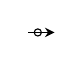
\begin{tikzpicture}[baseline=-0.6ex]
                \draw [myarrow, {-\myarrowhead}]
                (0, 0) -- (2.2ex, 0);
                \draw (0.8ex,0) circle (0.3ex);
            \end{tikzpicture}%
          $}%
          }
}

\DeclareRobustCommand\myleftarrow{%
  \mathrel{%
    \mbox{$
            \begin{tikzpicture}[baseline=-0.6ex]
                \draw [myarrow, {\myarrowhead-}]
                    (0, 0) -- (2.0ex, 0);
            \end{tikzpicture}%
          $}%
          }
}

\DeclareRobustCommand\myleftrightarrow{%
  \mathrel{%
    \mbox{$
            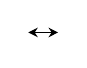
\begin{tikzpicture}[baseline=-0.6ex]
                \draw [myarrow, {\myarrowhead-\myarrowhead}]
                    (0, 0) -- (2.5ex, 0);
            \end{tikzpicture}%
          $}%
          }
}


\newcommand{\gdtt}{\ensuremath{\sym{GDTT}}\xspace}
\newcommand{\gctt}{\ensuremath{\sym{GCTT}}\xspace}
\newcommand{\modalfrp}{\ensuremath{\sym{ModalFRP}}\xspace}

\newcommand\bnfeq{::=}
\newcommand\kleq{\simeq}%kleene equality
\newcommand\sym[1]{\mathsf{#1}}
\newcommand\fix[1]{\sym{fix}^{#1}}
\newcommand\dfix[1][\kappa]{\sym{dfix}^{#1}}
\newcommand\nxt[1][\kappa]{\sym{next}^{#1}}
\newcommand\tabs[2]{\lambda (#1 : #2).}
\newcommand\tickc{\diamond}
%anonymous tick
\newcommand\tick[1][\rho]{
\ooalign{$\checkmark$\cr$^#1$\hss}}
\newcommand\tickA{\alpha}
\newcommand\tickB{\beta}
\newcommand\tapp[2][\tickA]{#2\ [#1] }
\newcommand\tappc[1]{\tapp[\tickc]{#1}}
\newcommand\adv[1][]{\sym{adv}^{#1}}
\newcommand\delay[1][]{\sym{delay}^{#1}}
\newcommand\rbox[1][]{\sym{box}^{#1}}
\newcommand\unbox[1][]{\sym{unbox}^{#1}}
\newcommand\vinterp[2][\rho_E,\rho_N]{\mathcal{V}\llbracket #2 \rrbracket_{#1}}
\newcommand\einterp[2][\rho_E,\rho_N]{\mathcal{E}\llbracket #2 \rrbracket_{#1}}
\newcommand\frplat[1][]{\ensuremath{{\bigcirc}^{#1}}}
\newcommand\frpbox[1][]{\ensuremath{{\Box}^{#1}}}
\newcommand\unlock{\CheckedBox}
\newcommand\open[1]{\sym{open} \; #1}
\newcommand\shut[1]{\sym{shut} \; #1}
\newcommand\push[1]{\sym{push} \; #1}
\newcommand\pull[1]{\sym{pull} \; #1}

%\newcommand\foldI[1][F]{\sym{fold}_{\foldT}}
% \newcommand\fold[1]{\sym{fold}_{#1}}
%\def\foldT{#1}
%\foldI
%}
% \newcommand\foldc{\fold}
%\newcommand\unfoldI[1][F]{\sym{unfold}_{\unfoldT}}
% \newcommand\unfold[1]{\sym{unfold}_{#1}}
%\def\unfoldT{#1}
%\unfoldI
%}
% \newcommand\unfoldc{\unfold[{\tickc}]}

\newcommand\eqmodcl{\approx}

\newcommand\refrule[1]{\textsc{#1}}

\newcommand\defeq{\mathrel{:=}}


\newcommand\sat{\ensuremath{\mathsf{Sat}}\xspace}

\newcommand\ds[1]{\left[#1\right]}
\newcommand\bind[2]{#1\leftarrow #2}
\newcommand\dss[2]{\ds{#1}_{#2}}
\newcommand\prev[1][\kappa]{\sym{prev}{#1}.}
\newcommand\app[1][\kappa]{\mathrel{\circledast^{#1}}}
\newcommand\fv[1]{\sym{fv}(#1)}
\newcommand\ft[1]{\sym{ft}(#1)}
\newcommand\ftc[1]{\sym{ft}^*(#1)}
\newcommand\fc[1]{\sym{fc}(#1)}
\newcommand\bv[1]{\sym{bv}(#1)}
\newcommand\bc[1]{\sym{bc}(#1)}

\newcommand\disj{\mathrel{\#}}


\newcommand\kripke{\ensuremath{{\mathcal K}}\xspace}

\newcommand\pair[2]{\left\langle#1,#2\right\rangle}

\newcommand\clockc{\kappa_0}
\newcommand{\clockkind}{{\small{\sym{c}}}}
\newcommand{\grclock}{{\small{\sym{grclock}}}}
\newcommand{\frpclock}{\sym{frpclock}}
\newcommand{\Fix}{\sym{Fix}\,}
\newcommand{\interm}{\sym{in}}
\newcommand{\caseterm}[5]{\sym{case}\, #1 \, \sym{of}\, \interm_1(#2) . #3 ; \interm_2(#4) . #5}
\newcommand{\letterm}[3]{\sym{let}\, #1 \, = #2 \, \sym{in} \, #3}
\newcommand{\commfp}{\sym{comm}_{\forall,+}}
\newcommand{\stream}[1]{S_{\frplat}^\kappa (#1)}
\newcommand{\gstream}[1]{S^\kappa (#1)}
\newcommand{\rstream}[1]{S_{\frplat} (#1)}


\newcommand\nats{{\mathbb N}}
\newcommand\Str{\sym{Str}}
\newcommand\gStr[1][\kappa]{\sym{Str}^{#1}}
\newcommand\fStrI[1][\kappa]{\sym{Str}^{#1}_{\fStrL}}
\newcommand\fStr[1][\tickA]{
\def\fStrL{#1}
\fStrI
}
\newcommand\gcons[1][\kappa]{\sym{cons}^{#1}}
\newcommand\gconst[1][\kappa]{\sym{const}^{#1}}
\newcommand\gtl[1][\kappa]{\sym{tl}^{#1}}
\newcommand\ghd[1][\kappa]{\sym{hd}^{#1}}
\newcommand\cons{\sym{cons}}
\newcommand\const{\sym{const}}
\newcommand\tl{\sym{tl}}
\newcommand\hd{\sym{hd}}
\newcommand\nth{\sym{nth}}
\newcommand\Nat{\sym{Nat}}
% \newcommand{\latkap}[1]{foooooooooo}
\newcommand\latkap[1][\kappa]{\ensuremath{{\rhd}^{#1}}}
\newcommand\later{\ensuremath{\ \rhd\hspace{-0.3em}}}
\newcommand\latbind[2]{{\rhd}\, (#1:#2) .}
\newcommand\clat[1][\kappa]{\ensuremath{{\hat\rhd}^{#1}}}
\newcommand\clater{\ensuremath{{\hat\rhd}}}
\newcommand\clatbind[2]{\hat{\rhd}\, (#1:#2) .}
\newcommand\ctimes{\mathrel{\hat\times}}
\newcommand\cto{\mathrel{\hat\to}}

\newcommand\Bool{\sym{Bool}}
\renewcommand\tt{\sym{true}}
\newcommand\ff{\sym{false}}
\newcommand\ite{\sym{if}}
\newcommand\suc{\sym{suc}\,}
\newcommand\zero{\sym{0}}
\newcommand\pos[1]{{\mathcal P}os\left(#1\right)}
\newcommand\emptyseq{\langle\rangle}
\newcommand\cat{\cdot}
\newcommand{\id}[0]{\sym{id}}

\newcommand\decr[1]{\left[#1-\right]}

\newcommand\subterm[2]{#1\restriction{#2}}
\newcommand\parto{\rightharpoonup}


\newcommand\injto{\hookrightarrow }

\newcommand\sred{\mathrel{\hat\red}}

\newcommand\red{\myarrow}
\newcommand\redinv{\myleftarrow}
\newcommand\redequiv{\myleftrightarrow^*}
\newcommand\nfred{\red^*_{\mathsf{nf}}}
\newcommand\whred{\red_{\mathsf{WH}}}
\newcommand\whtopred{\mapsto}
\newcommand\whclo[2][\Delta]{#2^{\sym{wh}(#1)}}


\newcommand\CV{\sym{CV}}
\newcommand\TV{\sym{TV}}
\newcommand\Var{\sym{Var}}

\newcommand\pto{\rightharpoonup}
\newcommand\fpowerset[1]{{\mathcal P}_{\mathrm{fin}}(#1)}
\newcommand\subsetfin{\subseteq_{\mathrm{fin}}}

\newcommand\wflab[2][\Delta]{#2 \vdash_{#1}}
\newcommand\wfindex[2][\LL]{#2 \vdash^{#1}}
\newcommand\wfcxt[2][\Delta]{#2 \vdash_{#1}}
\newcommand{\wfclock}[3]{#2\vdash_{#1} #3 \,: \,\sym{clock}}


\newcommand\tokens[1]{\sym{Tok}\left(#1\right)}
\newcommand\weakty[3][\Delta]{#2\vdash_{#1}#3}
\newcommand\type{\sym{type}}
\newcommand\mset[1]{\left\{#1\right\}}
\newcommand\set[1]{\left\{#1\right\}}
\newcommand{\setcom}[2]{\set{#1\left\vert\vphantom{#1}\,#2\right.}}
\newcommand\hastype[4][\Delta]{
#2 \vdash_{#1} #3: #4
}

\newcommand\istype[3][\Delta]{
#2 \vdash_{#1} #3: \type
}

\newcommand\eqtypeII[4][\II]{
#2 \vdash^{\eqtypeL}_{\eqtypeD} #3 \simeq #4:_{#1} \type
}
\newcommand\eqtypeI[1][\LL]{
\def\eqtypeL{#1}
\eqtypeII
}
\newcommand\eqtype[1][\Delta]{
\def\eqtypeD{#1}
\eqtypeI}

\newcommand\sto[4]{{\wfcxt[#1]{#2}} \to {\wfcxt[#3]{#4}}}
\newcommand\subst[2]{\left[#1/#2\right]}
\newcommand\substd[4]{\left[#1/#2,#3/#4\right]}
\newcommand\toksubst[3][\kappa]{\left[#2/#3\right]}
\newcommand\capsubst[2]{\left\{#1/#2\right\}}
\newcommand\substs[3]{\subst{#1}{#2}_{#3}}
\newcommand\repl[2]{\left[#1 \mapsto #2\right]}
\renewcommand\|{\;|\;}


\newcommand\ol[1]{\overline{#1}}

\newcommand{\UU}{{\mathcal U}}
\newcommand\El[1]{\sym{El}\left(#1\right)}

\newcommand\DD{{\mathcal D}}
\newcommand\KK{{\mathcal K}}
\newcommand\LL{{\mathcal L}}
\newcommand\II{{\mathcal I}}
\newcommand\JJ{{\mathcal J}}
\newcommand\TT{{\mathcal T}}
\newcommand\OO{{\mathcal O}}
\newcommand\card[1]{\left|#1\right|}


\newcommand\semcxtII[1]{\left\llbracket #1 \vdash_{\semcxtD}
  \right\rrbracket_{\semcxtN}}

\newcommand\semcxt[1][\Delta]{
\def\semcxtD{#1}
\semcxtI
}

\newcommand\semcxtI[1][\sigma,\delta]{
\def\semcxtN{#1}
\semcxtII}


\newcommand\semlab[2]{\left\llbracket #2\right\rrbracket_{#1}}
\newcommand\semnat{{\mathcal N}}


\newcommand\semtyII[1]{\left\llbracket \vdash_{\semtyD} #1
  \right\rrbracket_{\semtyN}}

\newcommand\semty[1][\Delta]{
\def\semtyD{#1}
\semtyI
}


\newcommand\semtyI[1][\delta]{
\def\semtyN{#1}
\semtyII}



\newcommand\types{\mathsf{Types}}
\newcommand\dom[1]{\mathsf{dom}\left(#1\right)}
\newcommand\supp[1]{\mathsf{supp}\left(#1\right)}

\newcommand\tyvarmaps[1][\Theta]{\left\llbracket #1 \right\rrbracket}
\newcommand\tyvarmapssubst[2][\Theta]{\llbracket #1,#2 \rrbracket}

\newcommand\SN{\ensuremath{\mathsf{SN}}\xspace}
\newcommand\CSN{\ensuremath{\mathsf{CSN}}\xspace}

\newcommand\neutral{\sym{Neu}}

\newcommand\restr[2]{#1\restriction{#2}}

\newcommand\inl{\sym{inl}}
\newcommand\inr{\sym{inr}}

\newcommand\case{\mathsf{case}}

\newcommand\unit{\langle\rangle}
\newcommand\Unit{\sym{1}}
\newcommand\parred{\mypararrow}
\newcommand\binds[1]{\mathsf{dom}\left(#1\right)}


\newcommand{\comm}[3][red]{{\color{#1}{$\spadesuit$#2: #3}}}
\newcommand{\todo}[1]{\comm{TODO}{#1}}


% gDTT macros

\newcommand{\gdttlat}[3][\kappa]{\rhd^{#1}#2.#3}
\newcommand{\hrt}[1]{\left[ #1 \right]}
\newcommand{\typeeqrel}{\ensuremath{\equiv}}
\newcommand{\pure}[3][\kappa]{\nxt[#1]#2.#3}
\newcommand{\termeqrel}{\ensuremath{\equiv}}
\newcommand{\univcode}[1]{\widehat{#1}}
\newcommand{\gdttlatcode}[1]{\univcode{\rhd}^{#1}}

\newcommand{\dsubst}[5]{\ensuremath{\vdash_{#1} #3 : #4 \overset{#2}{\rightarrowtriangle} #5}}
\newcommand{\emptyctx}{\mathop{\cdot}}
\newcommand{\wftype}[3]{\ensuremath{#2 \vdash_{#1} #3 \, \operatorname{type}}}
\newcommand{\isclock}[2]{\ensuremath{\vdash_{#1} #2}}
\newcommand{\alwaystype}[2]{\ensuremath{\forall{#1}{.#2}}}
\newcommand{\dstocm}[3]{\operatorname{adv}_{#1}^{#2}(#3)}
\newcommand{\ctxmorph}[4]{\ensuremath{#2}}% :_{#1} #3 \to #4}}
\newcommand{\esubst}[2]{[#2/#1]} % explicit subst/ctx morph
\newcommand{\alwaysapp}[2]{\ensuremath{#1\!\left[#2\right]}} % eliminator
\newcommand{\termeq}[5]{\ensuremath{#2 \vdash_{#1} #3 \termeqrel #4 : #5}}
\newcommand{\alwaysterm}[2]{\ensuremath{\Lambda{#1}{.#2}}}
\newcommand{\gdtttrans}[1]{#1^*}

\newcommand\qkeep{\sym{keep}}
\newcommand\qdelete{\sym{delete}}
\newcommand\update[3]{[#1 \mapsto \heap{#2}{#3}]}

\newcommand\heap[2]{\pair{#1}{#2}}


% Comments
\newcommand{\rem}[1]{\textbf{REM} #1}

% for complete-easy inference
\newcommand{\checks}[0]{\mathbin{\textcolor{blue}{⇐}}}
\newcommand{\synths}[0]{\mathbin{\textcolor{red}{⇒}}}
\newcommand{\appsynths}[0]{\mathbin{\textcolor{OliveGreen}{⇒\hspace{-.5em}⇒}}}
\newcommand{\bull}[0]{\mathbin{\textcolor{OliveGreen}{∙}}}
\newcommand{\mathhuge}[1]{\mathlarger{\mathlarger{#1}}}
\newcommand{\subt}[0]{\mathbin{\textcolor{Fuchsia}{\code{<:}}}}
\newcommand{\ahat}[0]{\hat{α}}
\newcommand{\bhat}[0]{\hat{β}}
\newcommand{\instantiateLeft}[0]{\code{:=\raisebox{0.5em}{\hspace{-0.6em}<}}}
\newcommand{\instl}[0]{\mathbin{\textcolor{Fuchsia}{\instantiateLeft}}}

\newcommand{\instantiateRight}[0]{\,\code{{=\raisebox{0.5em}{\hspace{-0.6em}<}}}\hspace{-0.3em}:}
\newcommand{\instr}[0]{\mathbin{\textcolor{Fuchsia}{\instantiateRight}}}

\newcommand{\marker}[0]{{\scriptstyle ▶}}

% for clofrp specification
\newcommand{\stable}[0]{stable}
\newcommand{\patcheck}[0]{\mathbin{\textcolor{Bittersweet}{\swneharpoons}}}
\newcommand{\branchcheck}[0]{\mathbin{\textcolor{Emerald}{\Yleft\hspace{-0.5em}⇐}}}
\newcommand{\checkbranch}[4]{(#1\!:\!#2 ⟶ #3) \branchcheck #4}

\newcommand{\Decl}[0]{}
\newcommand{\rulename}[1]{\textsc{\mbox{\Decl#1}}}
\DeclareDocumentCommand{\afk}{ O{χ} O{} }{α\IfNoValueTF{#2}{}{_{#2}}\!:\!#1}
\DeclareDocumentCommand{\ahatk}{ O{χ} O{} }{\ahat\IfNoValueTF{#2}{}{_{#2}}\!:\!#1}
\DeclareDocumentCommand{\bhatk}{ O{χ} O{} }{\bhat\IfNoValueTF{#2}{}{_{#2}}\!:\!#1}
\newcommand{\hask}{\!:\!}
\newcommand{\karr}{\!\!→\!}
\newcommand{\alphas}[0]{\overrightarrow{α}}
\newcommand{\ahats}[0]{\overrightarrow{\hat{α}}}
\newcommand{\fixx}[0]{\sym{fix}}
\newcommand{\fold}[0]{\sym{fold}}
\newcommand{\unfold}[0]{\sym{unfold}}

\newcommand{\haskind}[0]{⤇}
\newcommand{\branch}[1]{ρ_{#1} ⟶ e_{#1}}
\newcommand{\fmap}[0]{\sym{fmap}}

\newcommand{\primRec}[0]{\sym{primRec}}
\newcommand{\alt}[0]{\,|\,}
\newcommand{\Strk}[0]{\textsf{Str}^κ}
\newcommand{\Strka}[0]{\textsf{Str}^κ_α}
\newcommand{\kind}[0]{\chi}
\newcommand{\clockk}[0]{\mathsf{c}}
\newcommand{\Type}[0]{\mathscr{T}}
\newcommand{\Constr}[0]{\mathscr{C}}
\newcommand{\Pat}[0]{\mathscr{P}}
\newcommand{\Rec}[0]{\mathsf{Fix}}
\newcommand{\tickabs}[0]{γ}

\newcommand{\eval}[0]{⇓}
\newcommand{\stepsem}[3]{#1 ⊢ #2 \mathbin{\textcolor{blue}{⇓}} #3}
\newcommand{\appsem}[4]{#1 ⊢ #2\; #3 \mathbin{\textcolor{OliveGreen}{⇊}} #4}
\newcommand{\patsem}[4]{#1 ⊢ #2 \mathbin{\textcolor{Bittersweet}{⇂}} #3 ⊣ #4}
\newcommand{\tickop}[0]{⋙}
\newcommand{\ticksem}[3]{#1 ⊢ #2 \mathbin{\textcolor{BrickRed}{\tickop}} #3}
\newcommand{\forceop}[0]{\lightning}
\newcommand{\force}[3]{#1 ⊢ #2 \mathbin{\textcolor{BurntOrange}{\forceop}} #3}
\newcommand{\clos}[3]{λ_{#1}\,#2.\ #3}
\newcommand{\tclos}[3]{γ_{#1}\,#2.\ #3}

\newcommand{\Maybe}[0]{\textsf{Maybe}}
\newcommand{\Nothing}[0]{\textsf{Nothing}}
\newcommand{\Just}[0]{\textsf{Just}}

\newcommand{\RuleForallL}[0]{\textsc{\ensuremath{≤\hspace{-0.3em}∀}L}\xspace}
\newcommand{\RuleArrowI}[0]{\ensuremath{→}\textsc{I}\ensuremath{\synths}\xspace}
\newcommand{\RuleForallApp}[0]{\textsc{\ensuremath{∀}App}\xspace}

\newcommand{\forallt}[0]{\mathsf{forall}}

\begin{document}
\begin{comment}
A major problem is how to present tick-application and normal application properly.
In the source code, they share the same abstract syntax, but we distinguish by wrapping
tick-variables and tick-constants in brackets.
So e1 e2 is `App e1 e2` and e1 [e2] is `App e1 (TickVar e2)`.
But the presentation only has syntax e1 e2 and e1 [e2], so (TickVar e2) so not exist as
syntax. Because of that, we cannot use the presentation of the algorithmic inference rules
in its current form, as it refers to non-existant syntax, since [x] and [♢] cannot stand
alone. So either, change the presentation-syntax to conform with the implementation, or
you will have to come up with new rule exactly like application-synthesis, but for ticks.
\end{comment}
\sloppy

%% Title information
\title[Productive Co-Programming in Haskell]{Productive Co-Programming in Haskell with Ticking Clocks}         %% [Short Title] is optional;
                                        %% when present, will be used in
                                        %% header instead of Full Title.
%\titlenote{with title note}             %% \titlenote is optional;
                                        %% can be repeated if necessary;
                                        %% contents suppressed with 'anonymous'
% \subtitle{Subtitle}                     %% \subtitle is optional
% \subtitlenote{with subtitle note}       %% \subtitlenote is optional;
                                        %% can be repeated if necessary;
                                        %% contents suppressed with 'anonymous'


%% Author information
%% Contents and number of authors suppressed with 'anonymous'.
%% Each author should be introduced by \author, followed by
%% \authornote (optional), \orcid (optional), \affiliation, and
%% \email.
%% An author may have multiple affiliations and/or emails; repeat the
%% appropriate command.
%% Many elements are not rendered, but should be provided for metadata
%% extraction tools.

%% Author with single affiliation.
\author{Adam Schønemann}
                                        %% can be repeated if necessary
\affiliation{
  \position{Msc Graduate}
  % \department{Computer Science}              %% \department is recommended
  \institution{IT University of Copenhagen}            %% \institution is required
  \streetaddress{Rued Langgaards Vej 7}
  % \city{Copenhagen S}
  % \postcode{2300}
  \country{Denmark}                    %% \country is recommended
}
\email{adsc@itu.dk, adamschoenemann@gmail.com}          %% \email is recommended

%% Abstract
%% Note: \begin{abstract}...\end{abstract} environment must come
%% before \maketitle command
\begin{abstract}
Guarded recursion allows a form of general recursion to be
added to a language without breaking consistency. Consistency is especially important for
proof-assistants, but is also a useful property for safe general-purpose programming. Guarded
recursion has proven a natural fit for the domain of FRP (functional reactive programming),
since FRP programs are inherently required to be both causal and productive; both properties
are elegantly ensured by guarded recursion. Recently, several type theories based on guarded
recursion have emerged, one of which is \clott (Clocked Type Theory). \clott uses guarded recursion to also type definitions
that are \textit{acausal} yet productive, by using \textit{clock variables} and \textit{clock quantification}.
Thus, it extends the set of definitions that can be
typed while still ensuring consistency in the context of proof-assistants. This paper
presents an implementation of the simply-typed fragment of \clott which is aimed at practical
programming with both inductive, guarded recursive and coinductive types. We expand the calculus with
useful constructs; design and implement a modern type inference system with user-definable
types; design a big-step operational semantics and a compilation scheme targeting Haskell.
We conclude that productive practical coprogramming with clocks is realizable without
sacrificing significant programmer ergonomics or introducing prohibitive complexity into the
theory or the implementation of existing languages.
\end{abstract}


%% 2012 ACM Computing Classification System (CSS) concepts
%% Generate at 'http://dl.acm.org/ccs/ccs.cfm'.
\begin{CCSXML}
<ccs2012>
<concept>
<concept_id>10011007.10011006.10011008</concept_id>
<concept_desc>Software and its engineering~General programming languages</concept_desc>
<concept_significance>500</concept_significance>
</concept>
</ccs2012>
\end{CCSXML}

\ccsdesc[500]{Software and its engineering~General programming languages}
%% End of generated code


%% Keywords
%% comma separated list
\keywords{functional programming, guarded recursion, clock variables}  %% \keywords are mandatory in final camera-ready submission


%% \maketitle
%% Note: \maketitle command must come after title commands, author
%% commands, abstract environment, Computing Classification System
%% environment and commands, and keywords command.
\maketitle


\section{Introduction}
Lazy evaluation, as popularized by Haskell, allows us to express and
compose infinite programs that still yield useful output. Under lazy evaluation, an infinite program is
\emph{productive} if it produces output for any finite ``point in time''. \code{zeros = 0 : zeros} is productive, while \code{xs = xs} is
not. Non-productive programs are unresponsive, and correspond to a proof of \textit{False} in the Curry-Howard
interpretation, and therefore we wish to exclude such programs statically. Infinite programs can
also be \emph{causal}. A causal definition produces output at time $n$ by examining input only
from time $m$ where $m ≤ n$.
For example, \code{noncausal (x : y : xs) = y : noncausal xs}
will always depend on a future value before producing any output, and thus
cannot produce output in the current time-step. If the input to \code{noncausal} is being
constructed ``at the same time'' as \code{noncausal} produces output, then the program will
hang. As a concrete example \footnote{Which McBride learned of from Nils Anders Danielsson
in \url{https://mazzo.li/epilogue/index.html\%3Fp=186.html}}
from Atkey \& McBride \cite{atkey2013productive}, consider the two following
definitions of \code{map} on infinite streams in Haskell:

\begin{minted}{haskell}
data Stream a = Cons a (Stream a)
map, maap :: (a -> b) -> Stream a -> Stream b
map f (Cons x xs) = Cons (f x) (map f xs)
maap f (Cons x1 (Cons x2 xs)) =
  Cons (f x1) (Cons (f x2) (maap f xs))
\end{minted}

If applied to fully constructed streams, their behaviour is identical. But if applied to
streams that are still ``being constructed'', \code{maap} can diverge while \code{map} executes as expected for any stream. For example:

\begin{minted}{haskell}
data Stream a = Cons a (Stream a)
nats = Cons 0 (map (+ 1) nats)
badnats = Cons 0 (maap (+ 1) badnats)
\end{minted}

\code{nats} produces the infinite stream of natural numbers, but \code{badnats} diverges,
since \code{maap} requires two values to be available on the input stream but there ever
only is one. Since \code{nats} and \code{badnats} has the same type, their distinct
semantics is not captured adequately by their types.

\subsection{Guarded Recursion}\label{sec:guarded-recursion}
Guarded recursion was originally suggested by Nakano \cite{nakano2000modality}
to address the challenge of working with coinductive data in proof assistants.
Guarded recursion introduces a new modality $\rhd$, pronounced ``later'',
which makes it possible to distinguish between values we can use now, and
values we can only use later.
This distinction is exactly what is needed in order to ensure
causality, by constructing a type system that prohibits using ``later'' values
now. In the same way, guarded recursion ensures productivity, by requiring that
definitions return something ``now'' if they are to be used ``now''.
For example, the type of infinite streams would be expressed as \newline
\mintinline[mathescape=true,escapeinside=||]{haskell}
{data Stream a = Cons a |$\rhd$|(Stream a)} while the unrestricted fixpoint combinator
% use recursive types instead? μX. A × X.
is replaced with the guarded fixpoint
\mintinline[mathescape=true,escapeinside=||]{haskell}{fix :: (|$\rhd$|a -> a) -> a}.

Several approaches for using guarded recursion for functional reactive programming have been
proposed \cite{krishnaswami2011ultrametric,cave2014fair,simple-frp}. Since FRP deals primarily
with time-dependent data, guarded recursion seems to be a natural fit for FRP.

Guarded recursion is a simple and effective solution for writing infinite yet productive (and causal)
programs. The problem is that the world of guarded recursion is too restrictive for many domains.
We cannot make finite observations on guarded recursive data; as such we cannot type the following
definition:

\begin{minted}{haskell}
take :: Natural -> Stream a -> List a
take 0 _ = []
take (n + 1) (Cons x xs) = x : take n xs
\end{minted}

The problem arises because $\code{xs}$ has type $\later (\code{Stream a})$ in
the second clause,
whereas \code{take} expects its second argument to have type $\code{Stream a}$.
The global time-slicing of guarded recursion prevents us from ever looking into the ``future'',
even on fully-constructed data. This is by design, but once data has been constructed, we should
be able to scrutinize its structure as far as desired. Atkey \& McBride \cite{atkey2013productive} solve this
problem by \textit{localizing} the conceptual time-line that data is being constructed on
using the concept of \textit{clock variables}.

\subsection{Clock variables}
A clock variable represents a time-line that can be used for constructing guarded recursive
data. As such, the guardedness type constructor is now indexed by a clock variable $κ$.
Consequently, we can conceptually re-define the type of guarded streams as
\begin{minted}[mathescape=true,escapeinside=||]{haskell}
data Stream (|$κ$| :: Clock) (a :: *) = Cons a |$\rhd^κ$|(Stream |$κ$| a)
\end{minted}

The guarded fixpoint combinator is also indexed over a clock variable, and typed as

\begin{minted}[mathescape=true,escapeinside=||]{haskell }
fix :: |$∀$|(|$κ$| :: Clock). (|$\rhd^κ$|a -> a) -> a
\end{minted}

We can think of the guarded stream $\mathsf{Stream}\ κ\ a$ as being the type of ``streams in
construction'', whereas the clock quantified type $∀κ.\ \mathsf{Stream}\ κ\ a$ represents the
type of ``fully-constructed'' streams. Intuitively, a clock represents some time-line that
can be thought of as a resource to use for making finite observations on data. Thus, the
type $\mathsf{Stream}\ κ\ a$ represents streams on which we can only observe the head ``now'',
whereas the quantified type $∀κ.\ \mathsf{Stream}\ κ\ a$ says that for \textit{any} clock,
we can get a stream, and thus we can safely destructure the stream as much as we would like.
Atkey \& McBride \cite{atkey2013productive} also provide clock abstraction $Λκ. e$ and clock application
$e[κ]$ in the style of System F, as well as the type equality $∀κ.\, A ≡ A$ when $κ ∉ fv(A)$,
and the primitive $\mathsf{force} :: (∀κ.\, \rhd^κ A) → (∀κ.\, A)$. Using this, we can
write
\begin{minted}[mathescape=true,escapeinside=||]{haskell}
uncons :: (|$∀κ$|. Stream |$κ$| a) -> (a, |$∀κ$|. Stream |$κ$| a).
uncons xs =
  ( |$Λκ$|. case xs[|$κ$|] of Cons x _ -> x
  , force (|$Λκ$|. case xs[|$κ$|] of Cons _ xs -> xs[|$κ$|]))
\end{minted}

We can now type \code{take} for fully-constructed streams:
\begin{minted}[mathescape=true,escapeinside=||]{haskell}
take :: Natural -> (|$∀κ$|. Stream |$κ$| a) -> List a
take 0 _ = []
take (n + 1) xs = x : take n xs' where
  (x, xs') = uncons xs
\end{minted}

Using clock variables, we can only type \code{map} and \code{maap} above as
\begin{minted}[mathescape=true,escapeinside=||]{haskell }
map :: |$∀κ$|. (a -> b) -> Stream |$κ$| a -> Stream |$κ$| b
maap :: (a -> b) -> (|$∀κ$|. Stream |$κ$| a) -> (|$∀κ$|. Stream |$κ$| b)
\end{minted}

Their types clearly reflect their behaviour, namely that \code{maap} is only defined for
fully-constructed streams, which allows us to statically rule out programs
such as \code{badnats}.

Bahr et al. \cite{bahrclocks} extended the work of AtKey \& McBride to a dependent type-theory
called \clott and gave a strongly normalizing reduction semantics by introducing \textit{ticks}
on clocks $α : κ$ and the \textit{tick constant} $\tickc$, along with tick abstraction $λ(α : κ).\ e$
and application $e[α]$. The guarded type modality is extended to a dependent version as
$\latbind{α}{κ}\, A$. If $α$ is not free in $A$ we simply write $\latkap A$.
A term of such a type can be forced by applying it to the tick constant
$\tickc$, which in general is unsafe: $λ(x : \latkap A).\, x[\tickc]$ is for example not productive
and should not be typeable. But it is safe to force an open term if $κ$ is not free in the
context, leading to the rule\footnote{The rule is not the actual rule for tick constant application
(which is more complicated), as it is not closed under substitution or weakening, but it is admissible.}:

\begin{mathpar}
\inferrule{Γ ⊢_{∆,κ} e : \latbind{α}{κ}\, A \and Γ ⊢_∆}
          {Γ ⊢_{∆,κ} e[\tickc] : A[\diamond/α]}
\end{mathpar}

Here, the typing judgment $Γ_Δ ⊢ e : A$ is subscripted with a clock-context $Δ$ containing all introduced
clock variables. As such, the rule states that applying the tick constant to a suspended computation
on clock $κ$ is only well-typed if the context is well-typed \textit{without} $κ$; that is, a
context where $κ$ is not free. Such a context is called $κ$-stable. The effect is that the
tick constant cannot be used to force a suspended computation over $κ$ under any tick abstractions
over $κ$, and as such a fixpoint can only be unfolded once with a tick constant.

There is to our knowledge no implementation of a language with clock variables. Although
the theory is sound, it can be hard to predict how they integrate in a practical setting:
do they interfere with type inference? Can they be used ergonomically? What are their
implementation strategies? We seek to explore this space by implementing an
embedded language in Haskell designed for practical programming. Its theory is based on the
simply-typed fragment of \clott.

\subsection{Our contributions}
\begin{itemize}
  \item We present \clopl, a language for co-productive programming
        based on Bahr et al. \cite{bahrclocks}. The semantics is given by a coinductively defined
        big-step operational semantics. The type system
        ensures that all CloPL programs are productive and thus have a well-defined
        semantics.
  \item We derive a higher-rank type inference algorithm for \clopl by adapting the work of
        Dunfield \& Krishnaswami \cite{dunfield2013complete} to a guarded recursive setting.
  \item We implement \clopl as an embedded language in Haskell using quasi-quotation.
  \item In addition to a direct implementation of the operational semantics,
        we provide an efficient implementation of \clopl by compiling it into
        Haskell.
  \item We present some examples illustrating the practical use of \clopl.
\end{itemize}

Our implementation of \clopl, along with example programs, is available
at \url{https://github.com/adamschoenemann/clofrp}.

\section{\clopl}\label{sec:clopl}
\clopl (Clocked Programming Language) is based on the theoretical foundation
of the simply-typed fragment of \clott. While \clopl is a research language it aims to explore
clock quantification and guarded recursion in a practical setting, so it aims to include many
modern programming language features such as parametric polymorphism, type inference,
user-defined algebraic data-types, pattern-matching, higher-rank and higher-kinded types,
type-synonyms and code deriving.
It does \textit{not} include general recursion, as that would defeat the purpose of
guarded recursion; instead, it provides a primitive recursion combinator and a guarded
fixpoint combinator.

\subsection{Type system}
\begin{figure}
$$
\begin{array}{lrll}
\text{Types} & A,B,F & ::= & X \alt A → B \alt \Fix X.\, F \alt \latkap\, A \\
\text{Terms} & e & ::= & x \alt λ(x : A). e \alt λ(α : κ).\, e \alt \\
 &  &                  & e_1\, e_2 \alt e\, [α] \alt e\, [\tickc] \alt e\, [κ] \alt \sym{fix} \alt \\
 &  &                  & \tickc \alt \sym{fold} \alt \sym{unfold} \alt \primRec_{F} \\
\text{Contexts} & Γ & ::= & ⋅ \alt  Γ, x : A \alt Γ, α : κ \\
\text{Clock Contexts} & Δ & ::= & ⋅ \alt  Δ, κ
\end{array}
$$
\caption{Selected grammar rules from simply-typed \clott.}
\label{fig:sclott:grammar-rules}
\end{figure}

Figures \ref{fig:sclott:grammar-rules} and \ref{fig:sclott:rules} show selected syntax\footnote{Rules for e.g.
sums and products are left out.} and
typing rules for the core calculus of \clopl, which is based heavily on the simply-typed fragment of
\clott. The syntax is entirely standard except for tick abstraction $λ(α : κ).\, e$, tick application $e\, [α]$,
and clock application $e\, [κ]$.
Contexts come in two kinds: ordinary typing contexts $Γ$, which can both contain
assertions about the type of names, but also the clocks of ticks; and clock-contexts
$Δ$ which are simply lists of clock variables.
The $\latbind{α}{κ}\, A$ term from \clott is gone, since types can no longer depend on values, and therefore
they cannot depend on ticks either, and replaced with the ``ordinary'' clock-indexed guarded
type-former $\latkap A$.

Recursive types are modeled using the \textsf{Fix} type constructor, along with the \textsf{fold} and \textsf{unfold}
combinators which are similar to the traditional treatment of isorecursive types.
Notice that neither the \textsf{Fix} type or its (un)foldings directly mention any clock variables --
it is simply through the \textsc{Fix} rule that their guarded nature arises, since the
premise requires $e$ to have type $\latkap{A} → A$. The formation rules for recursive types
are predicated on the well-formedness of $\Fix X.\, A$; namely that $X$ can only occur strictly
positively \textit{unless} it is guarded by a $\latkap$ \cite{nakano2000modality}.

% TODO: Fix Unfold and Fold which use simply Γ ⊢ (not subscript) in their premises
\begin{figure*}
\begin{mathpar}
  \inferrule*[lab=Var]
  {\wfcxt{Γ,x:A,Γ'}}
  {\hastype{Γ,x:A,Γ'}{x}{A}}

  \and
  \inferrule*[lab=Abs,leftskip=2em]
  {\hastype{Γ, x : A}{e}{B}}
  {\hastype{Γ}{\lambda (x : A).\ e}{A \to B}}

  \and
  \inferrule*[lab=App,leftskip=2em]
  {\hastype{Γ}{e}{A \to B}\\
    \hastype{Γ}{s}{A}}
  {\hastype{Γ}{e\,s}{B}}

  \and
  \inferrule*[lab=TickAbs,leftskip=2em]
  {\hastype{Γ,\tickA:κ}{e}{A}  \\ κ ∈ Δ }% \\ \wfclock{Δ}{Γ}{κ}}
  {\hastype{Γ}{\tabs{\tickA}{κ}\ e}{\latkap A}}

  \and
  \inferrule*[lab=ClockAbs]
  {\hastype[Δ, κ]{Γ}{e}{A}\\
    \wfcxt{Γ}}
  {\hastype{Γ}{Λκ.\ e}{∀ κ.\ A}}

  \and
  \inferrule*[lab=ClockApp,leftskip=2em]
  {\hastype{Γ}{e}{∀ κ.\ A}\\
    κ' ∈ Δ}
  {\hastype{Γ}{e\ [κ']}{A \subst{κ'}{κ}}}

  \and
  \inferrule*[lab=TickApp,leftskip=2em]
  {\hastype{Γ}{e}{\latkap A}\\\wfcxt{Γ'}}
  {\hastype{Γ,\tickA: κ,Γ'}{\tapp[\tickA] e}{A}}

  \and
  \inferrule*[lab=TConstApp,leftskip=2em]
  {\hastype[Δ,κ]{Γ}{e}{\latkap A}\\ \wfcxt{Γ}}
  {\hastype[Δ,κ]{Γ}{\tappc{e}}{A}}

  \and
  \inferrule*[lab=Fix]
  {\hastype{Γ}{e}{\latkap{A} \to A} \\ κ \in Δ}
  {\hastype{Γ}{\fix{κ}\,e}{A}}

  \and
  \inferrule*[lab=Unfold,leftskip=4em]
  {\hastype{Γ}{e}{\Fix X.\, A} \\ Γ ⊢ \Fix X. A}
  {\hastype{Γ}{\unfold\,e}{A\subst{\Fix X. A}{X}}}

  \and
  \inferrule*[lab=Fold,leftskip=4em]
  {\hastype{Γ}{e}{A\subst{\Fix X. A}{X}} \\ Γ ⊢ \Fix X. A}
  {\hastype{Γ}{\fold\,e}{\Fix X. A}} \\

  \and
  \inferrule*[lab=PrimRec]
  {\hastype{Γ}{e}{F[(\Fix X.\, F[X]) × A] → A }}
  {\hastype{Γ}{\primRec_F\, e}{(\Fix X.\, F[X]) → A}}
\end{mathpar}

\caption{Selected typing rules from simply-typed \clott.}
\label{fig:sclott:rules}
\end{figure*}

The rules in Figure \ref{fig:sclott:rules} show that we type clock quantification and
clock application in much the same way as ordinary type quantification in e.g. System F.
\textsc{TickAbs} describes how the \emph{later}-type is introduced through tick abstraction,
while \textsc{TickApp} shows the elimination form.
The main difference is the guarded fixpoint \textsc{Fix} which is indexed over a clock $κ$,
and the tick constant application rule \textsc{TConstApp} whose second premise $Γ ⊢_Δ$
expresses that $Γ$ should be $κ$-stable by asserting that it is well-formed in a clock-context
without $κ$.

In this calculus we would represent natural numbers as
$\Nat := \Fix X.\, 1 + X$ and guarded streams as $\Strk := \Fix X.\, \Nat × \latkap X$,
giving rise to definitions:
$$
\begin{array}{rll}
\gcons  &: & \Nat → \latkap \Strk → \Strk \\
\gcons  &:=& λ(x : \Nat).\, λ(xs : \latkap \Strk).\, \fold\ ⟨x, xs⟩ \\
\ghd    &: & \Strk → \Nat \\
\ghd    &:=& λ(x : \Strk).\ \textsf{fst}\ (\unfold\ x) \\
\gtl    &: & \Strk → \latkap \Strk \\
\gtl    &:=& λ(xs : \Strk).\ \textsf{snd}\ (\unfold\ xs) \\
\gconst &:=& λ(n : \Nat).\ \fixx^κ (λ(g : \latkap \Strk).\ \gcons\ n\ g)
\end{array}
$$
We can then use universal quantification over clocks to model coinductive types from
guarded recursive types as per Atkey \& McBride \cite{atkey2013productive} to define
the type of coinductive streams $\Str := ∀κ.\, \Strk$ and then lift $\gconst$ to produce
coinductive streams as $\const := λ(n : \Nat).\, Λκ.\, \gconst\, n$. We can then lift
$\ghd$ and $\gtl$ in the same way. Here, we work in a context with a \textit{clock constant}
$κ_0$ which is used to instantiate a clock quantified value, thus safely removing the
guardedness. We then use primitive recursion to define the $\nth$ function
on streams:
$$
\begin{array}{rll}
\hd   &: & \Str → \Nat \\
\hd   &:=& λ(xs : \Str).\, \ghd[κ_0]\; (xs\; [κ_0]) \\
\tl   &: & \Str → \Str \\
\tl   &:=& λ(xs : \Str).\, Λκ.\, \gtl\; (xs\; [κ])\; [\tickc] \\
\nth  &: & \Nat → \Str → \Nat \\
\nth  &:=& \primRec_{1 + X}\, ( \\
  & & \quad λ(n : \Nat).\ λ(xs : \Str).\ \\
  & & \quad\quad \case\ \unfold\ n\ \sym{of} \\
  & & \quad\quad\quad \inl\, \unit ⟶ \hd\, xs \\
  & & \quad\quad\quad \inr\, ⟨n', rec⟩ ⟶ rec\; (\tl\; xs) \\
  & &)
\end{array}
$$

The calculus we have now presented illustrates the core mechanism of clock variables which
is central to \clopl, but it is not feasible to write practical programs with it alone. To do this,
we shall augment the calculus with higher-rank polymorphism, user-defined algebraic data-types,
higher-kinded types, pattern-matching and a bidirectional inference system.

\section{Type inference}
Our type inference leans heavily on that presented by Dunfield \& Krishnaswami
\cite{dunfield2013complete}, which is a bidirectional inference system for higher-rank
predicative polymorphism, with arbitrarily-deep quantifiers, which is (relatively) easy to implement
and specify, and retains the $η$-law (namely that if $(λx.\ f\, x) : A$ and $x ∉ FV(f)$, then $f : A$).
Dunfield \& Krishnaswami present their inference system in two forms: A declarative system,
that employs an oracle but which is simple and easy to understand; and a an algorithmic system,
which directly yields an algorithm, but is more complicated. They prove that their algorithmic
system is sound and complete wrt. their declarative system. We shall follow the same structure:
first we present a declarative specification of \clopl and then we follow the same procedure
as Dunfield \& Krishnaswami to derive the algorithmic specification. For a thorough account
of their approach, we refer the reader to their paper.

\subsection{Declarative inference for \clopl} \label{sec:inference:declarative}
The declarative inference system uses a bidirectional approach with a synthesis ($Ψ ⊢ e \synths A $) and
a checking judgment ($Ψ ⊢ e \checks A$). As in \cite{dunfield2013complete}, we add a third \emph{application synthesis} judgment
$Ψ ⊢ A \bull e \appsynths C$ that says if a (possibly polymorphic) function of type $A$
is applied to $e$, then the application synthesizes type $C$.

\subsubsection{Syntax}\label{sec:inference:declarative:syntax}
The syntax of \clopl can be seen in Figure \ref{fig:clopl:declarative:syntax}, specified
as an EBNF grammar.

\begin{figure*}
$$
\def\arraystretch{1.5}
\begin{array}{lrcl}
% add sidenote to disallow clock kinds directly to the right of arrows
\text{Kinds} & \kind & ::= & ⋆ \alt \clockk \alt \kind → \kind' \\
             & \kind' & ::= & ⋆ \alt \kind → \kind' \\
\text{Types} & A,B,C,F,G & ::= & \Type \alt A → B \alt ⟨A_1, \dots, A_n⟩ \alt α \alt ∀α\!:\!\kind.\, A
                        \alt F\, B \alt \Rec\, F \alt \latkap\, A \\
\text{Monotypes} & τ, σ & ::= & \Type \alt τ → σ \alt ⟨τ_1, \dots, τ_n⟩ \alt τ\, σ \alt α
                           \alt \Rec\, τ \alt \latkap\, τ \\
\text{Terms} & e & ::= & \hspace{-0.5em}
                    \begin{array}[t]{l}
                     x \alt \Constr \alt λx. e \alt e_1\, e_2 \alt ⟨e_1, \dots, e_n⟩ \alt (e : A)
                    \alt \tickabs(x : κ).\, e \alt e\, [x] \alt e\, \{A\} \alt \sym{fix}
                    \alt \sym{fold} \alt \sym{unfold} \alt \fmap_{F} \alt \primRec_{F} \\\hspace{-0.5em}
                    \alt \case\ e\ \sym{of}\ (\branch{1}, \dots, \branch{n}) \alt \letterm{ρ}{e_1}{e_2} % \\\hspace{-0.5em}
                    \end{array} \\
\text{Patterns} & ρ & ::= & x \alt \Constr\, ρ_1,\dots,ρ_n \alt ⟨ρ_1, \dots, ρ_n⟩ \\
\text{Contexts} & Ψ & ::= & \hspace{-0.5em}
                        \begin{array}[t]{l}
                        ⋅ \alt Ψ,x :_λ A \alt Ψ,x :_= A \alt Ψ,\Constr : A \alt Ψ,α : χ \alt Ψ,\Type : χ
                        \alt Functor(F)
                        \end{array}
\end{array}
$$

\caption{The syntax of the declarative specification of \clopl.}
\label{fig:clopl:declarative:syntax}
\end{figure*}

\paragraph*{Kinds} are either the inhabited kind $⋆$, the kind of clocks $\clockk$, or
the kind of type constructors $χ → χ'$. $χ'$ doesn't include the kind of clocks, since we
cannot have clocks that are indexed over anything. Thus, a clock-kind directly to the right
of an arrow is not valid syntax. $\clockk → ⋆$ is valid, as is $(\clockk → ⋆) → ⋆$,
but $⋆ → \clockk$ or $(⋆ → \clockk) → ⋆$ is not.

\paragraph*{Possibly polymorphic types} can be the name of a declared type $\Type$ in the set
of declared types. Examples could be \textsf{Nat} or \textsf{Unit}. We loosely
use the symbols $A,B,C$ to refer to types of kind $⋆$, and $F,G$ to refer to type constructors
of kind $χ → χ$. We have the
standard function space and n-ary tuples of types. $α$ signifies the use of a quantified
type variable, and are thus not related to ticks anymore, to avoid ambiguity.
Universal quantification of types mentions the kind of the quantified type
in $∀α : χ.\ A$, however we omit the kind and write $∀α.\ A$ when we mean $∀α : ⋆.\ A$.
Types can be applied to other types, written $F\, B$. We choose to represent
recursive types as a built-in type constructor \textsf{Fix}. Finally, we have the type of
delayed computations on clock $κ$ written $\latkap A$. Crucially, clock variables are just
normal type variables of kind $\clockk$, and so do not have any special syntatic form.
\textbf{Monotypes} are just normal types without quantification.

\paragraph*{Terms} are variables, constructor names $\Constr$ (e.g. $\sym{Nil}$ or $\sym{Cons}$), lambda
abstractions, term applications, n-ary tuples, annotated terms, tick abstractions
$\tickabs(x : κ).\, e$, tick application $e\, [x]$, and explicit type applications $e\, \{A\}$. We model
clock application is just a specialized form of type application (with kind $\clockk$), in the
same way that we model clock abstraction using regular type abstraction. One thing that we have
omitted is the term-level syntax for clock abstraction ($Λκ. e$). Our type system will be able
to infer tick abstractions from the type of terms. We use new syntax for tick abstractions to
avoid ambiguity, since the form that \clott uses -- $λ(α : κ).\, t$ -- is too easy to confuse
with a normal lambda, and $α$ is used for polymorphism instead. $γ$ looks kind of like an
upside-down lambda, so the symbol does signify some relation with the original syntax.

Fixpoints $\sym{fix}$ are the guarded recursive fixpoints of simply-typed \clott. The
normal fixpoint has type $\sym{fix} : (A → A) → A$, whereas the guarded fixpoint has type
$\sym{fix} : (\latkap A → A) → A$.

We can fold and unfold recursive types and map over functorial type constructors $F$ with $\sym{fmap}_F$.

In the same way as in \cite{atkey2013productive,cave2014fair}, we use $\primRec_F$ to write
functions using primitive recursion. A primitive
recursion combinator allows us to express well-founded inductive definitions without a
sophisticated termination checker. The downside is that it is somewhat clunky to work with,
and that a considerable class of more complicated terminating recursive functions cannot be
encoded.

Finally, there are case expressions with lists of branches and let-expressions.
\textbf{Branches} are simply a pattern and an expression.

\paragraph*{Patterns} are simply name-bindings $x$, constructor-patterns $\Constr$ applied
to zero or more patterns, or n-ary tuple patterns $⟨ρ_1,\dots,ρ_n⟩$.

\paragraph*{Declarative contexts} are lists that carry contextual information used
for typing. Names can be associated to types in two ways: through a lambda abstraction as $x :_λ A$,
or through a let-binding or pattern-match as $x :_= A$. This is important when we judge a
context as $κ$-stable, since let-bound variables are ignored, as they are effectively
just substitutions and thus cannot break productivity.
Constructors are bound to types as $\Constr : A$; we use such bindings to both type
pattern-matches and constructor-applications.
Declared types are associated with a kind as $\Type : χ$, while type variables are
associated as $α : χ$. Finally, we assert that a type $F$ of kind $⋆ → ⋆$ is functorial as
$Functor(F)$.

We can only associate new names to types when going under lambda abstractions or encountering
let-bindings or case-expressions. Type variables can only be associated with a kind when going
under a quantified type. The remaining forms are not added or removed to the context during
typing. Usually, these forms are elaborated from declarations given by the programmer in a
pre-processing step before typing takes place.

\subsubsection{Kinds of types}\label{sec:inference:kinds}
Types in \clopl have kinds, and these kinds can be derived inductively over the structure of a type.
The derivation rules are quite standard; we show just two here, but the complete rules
can be found in Appendix \ref{app:decl-kind}.
The \textsc{Kind$\latkap$} rule demonstrates how to derive the kind
of a later type, which requires the superscript $κ$ to have the kind of clocks $\clockk$:

\begin{mathpar}
\inferrule*[lab=Kind$\latkap$]
{ Ψ ⊢ κ \haskind \clockk \\ Ψ ⊢ A \haskind ⋆ }
{ Ψ ⊢ \latkap{A} \haskind ⋆ }
\and
\inferrule*[lab=Kind$→$]
{ Ψ ⊢ A \haskind ⋆ \\ Ψ ⊢ B \haskind ⋆ }
{ Ψ ⊢ A → B \haskind ⋆ }
\end{mathpar}

Asking whether the type of a term is well-formed
amounts to asking whether it correctly derives a kind, and if the kind is what we expected,
which depends on the context (usually we expect $⋆$).
Note that the \textsc{Kind$→$} rule disallows functions on clock variables as specified in \cite{bahrclocks}.


\subsubsection{Subtyping}\label{sec:inference:subtyping}
As in \cite{dunfield2013complete}, a type $A$ is a subtype of $B$ if $A ≡ B$ or a
generalization of $B$. For example, $A ≤ A$ and $∀α. A ≤ B$ if we can instantiate $α$ with a
monotype $τ$ such that $[τ/α]A ≤ B$ (rule \RuleForallL).
The subtyping rules of \clopl are pretty much
identical to the declarative subtyping rules of \cite{dunfield2013complete},
except extended to work with the larger source language. Rule \textsc{$≤$\latkap} derives
a subtyping relation for the \emph{later} type constructor simply by proceeding
covariantly. Type application $F\, A$ also proceeds covariantly, while the function space
is contravariant, as expected.
\begin{mathpar}
\inferrule*[lab=$≤$\latkap]
{ Ψ ⊢ κ_1 ≤ κ_2 \quad Ψ ⊢ A ≤ B }
{ Ψ ⊢ \latkap[κ_1]\, A ≤ \latkap[κ_2]\, B }
\and
\inferrule*[lab=$≤\hspace{-0.3em}∀$L,leftskip=1.5em]
{ Ψ ⊢ τ \haskind χ \quad Ψ ⊢ [τ/α]A ≤ B }
{ Ψ ⊢ ∀α \hask χ.\, A ≤ B }
\end{mathpar}

The complete subtyping rules can be found in Appendix \ref{app:decl-subtyping}.

\subsubsection{Declarative inference rules}\label{sec:inference:decl-rules}
The inference rules for \clopl (Figure \ref{fig:inference:decl-rules-selected} shows selected rules,
see Appendix \ref{app:decl-rules} for the complete picture) again closely resemble those of \cite{dunfield2013complete}.
To accomodate our larger language, we also introduce two new judgments:
($Ψ ⊢ ρ \patcheck A ⊣ Ψ'$) checks a pattern $ρ$ against a type $A$ and returns an
\emph{output context} $Ψ'$ which extends $Ψ$ with all bindings in $ρ$;
($Ψ ⊢ \checkbranch{ρ}{A}{e}{B}$) checks a branch of a $\case$ expression with pattern
$ρ$ of type $A$ and body $e$ against a type $B$.

\begin{figure*}

$$
\def\arraystretch{1.2}
\begin{array}{l}
\mathlarger{\boxed{Ψ ⊢ e \checks A}}\ \text{Under context $Ψ$, $e$ checks against type $A$} \\
\mathlarger{\boxed{Ψ ⊢ e \synths A}}\ \text{Under context $Ψ$, $e$ synthesizes type $A$} \\
\mathlarger{\boxed{Ψ ⊢ A \bull e \appsynths C}}\
  \text{Under context $Ψ$, applying a function of type $A$ to $e$ synthesizes type $C$} \\
% \mathlarger{\boxed{Ψ ⊢ \checkbranch{ρ}{A}{e}{B}}} \
%   \text{Under context $Ψ$, check branch $(\branch{})$ with pattern-type $A$
%         and body-type $B$ } \\
% \mathlarger{\boxed{Ψ ⊢ ρ \patcheck A ⊣ Ψ'}}\
%   \text{Under context $Ψ$, check pattern $ρ$ with type $A$ yielding new context $Ψ'$}
\end{array}
$$
\begin{mathpar}
\mprset{sep=1em}
\inferrule*[lab=\Decl Var]
{(x : A) ∈ Ψ}
{Ψ ⊢ x \synths A}

\inferrule*[lab=\Decl Constr$\synths$,leftskip=1.5em]
{(\Constr : A) ∈ Ψ}
{Ψ ⊢ \Constr \synths A}

\and
\inferrule*[lab=\Decl Sub,leftskip=3.5em]
{Ψ ⊢ e \synths A \\ Ψ ⊢ A ≤ B}
{Ψ ⊢ e \checks B}

\and
\inferrule*[lab=\Decl Anno,leftskip=3.5em]
{Ψ ⊢ A \haskind ⋆ \\ Ψ ⊢ e \checks A }
{Ψ ⊢ (e : A) \synths A}

\and
\inferrule*[lab=\Decl $∀$I,leftskip=3.5em, rightskip=2em]
{ Ψ, α \hask χ ⊢ e \checks A}
{Ψ ⊢ e \checks  ∀α \hask χ.\ A}

\and
\inferrule*[lab=\Decl $→$I]
{ Ψ,x :_λ A ⊢ e \checks B }
{Ψ ⊢ λx.\, e \checks  A → B}

\and
\inferrule*[lab=\Decl $∀$App]
{ Ψ ⊢ τ \haskind χ \\ Ψ ⊢ [τ/α]A \bull e \appsynths C}
{ Ψ ⊢ (∀α \hask χ .\ A) \bull e \appsynths C}


\and
\inferrule*[lab=\Decl $→$I$\synths$]
{ Ψ ⊢ σ → τ \haskind ⋆ \\ Ψ, x :_λ σ ⊢ e \checks τ }
{ Ψ ⊢ λx.\, e \synths σ → τ }

\and
\inferrule*[lab=\Decl $→$E]
{ Ψ ⊢ e₁ \synths A \\ Ψ ⊢ A \bull e_2 \appsynths C }
{ Ψ ⊢ e₁\, e₂ \synths C }

\and
\inferrule*[lab=\Decl $→$App]
{ Ψ ⊢ e \checks A }
{ Ψ ⊢ (A → C) \bull e \appsynths C }


\and
\inferrule*[lab=\Decl $\latkap$I$\synths$]
{ Ψ ⊢ κ \haskind \clockk \\ Ψ,x :_λ κ ⊢ e \synths A }
{Ψ ⊢ γ(x : κ).\, e \synths \latkap A }

\and
\inferrule*[lab=\Decl $\latkap$App,right=$e ≠ \tickc$]
{ Ψ ⊢ κ \haskind \clockk \\ Ψ ⊢ e \checks κ }
{ Ψ ⊢ (\latkap\, A) \bull e \appsynths A }

\and
\inferrule*[lab=\Decl $\latkap$App$\tickc$]
{ Ψ ⊢ κ \haskind \clockk \\ \stable_κ(Ψ) }
{ Ψ ⊢ (\latkap\, A) \bull \tickc \appsynths A }

\and
\inferrule*[lab=\Decl TApp,leftskip=1em]
{ Ψ ⊢ e \synths ∀(α : χ).\ B \\ Ψ ⊢ A \haskind χ }
{ Ψ ⊢ e\, \{A\} \synths [A/α]B }

% \and
% \inferrule*[lab=\Decl Fix]
% { }
% { Ψ ⊢ \sym{fix} \synths ∀(κ \hask \clockk), α.\ (\latkap α → α) → α }

% \and
% \inferrule*[lab=\Decl Fmap]
% { Functor(F) ∈ Ψ }
% { Ψ ⊢ \sym{fmap}_F \synths ∀α, β.\ (α → β) → F\, α → F\, β }

\and
\inferrule*[lab=\Decl PrimRec,leftskip=4em]
{ Functor(F) ∈ Ψ }
{ Ψ ⊢ \sym{primRec}_F \synths ∀α.\ F\, ⟨\Rec\, F, α⟩ → \Rec\, F → α }

% \and
% \inferrule*[lab=\Decl Case]
% { Ψ ⊢ e \synths A \\ Ψ ⊢ τ \haskind ⋆ \\ Ψ ⊢ A ≤ τ \\ Ψ ⊢ \checkbranch{ρ_1}{τ}{e_1}{B}
%   \ \dots \
%   Ψ ⊢ \checkbranch{ρ_n}{τ}{e_n}{B}
% }
% { Ψ ⊢ \case\ e\ \sym{of}\ (\branch{1}, \dots, \branch{n}) \checks B }

% \and
% \inferrule*[lab=\Decl Branch]
% { Ψ ⊢ ρ \patcheck A ⊣ Ψ' \\ Ψ' ⊢ e \checks B }
% { Ψ ⊢ \checkbranch{ρ}{A}{e}{B} }

% \and
% \inferrule*[lab=\Decl PatTuple]
% { Ψ ⊢ ρ_1 \patcheck A_1 ⊣ Ψ_1 \ \dots \ Ψ_{n-1} ⊢ ρ_n \patcheck ⊣ Ψ_n }
% { Ψ ⊢ ⟨ρ_1, \dots, ρ_n⟩ \patcheck ⟨A_1, \dots, A_n⟩ ⊣ Ψ_n }

% \and
% \inferrule*[lab=\Decl PatBind]
% { }
% { Ψ ⊢ x \patcheck A ⊣ Ψ, x :_= A }

% \and
% \inferrule*[lab=\Decl PatConstr]
% { (\Constr : A') ∈ Ψ  \and
%   Ψ ⊢ ρ_1 \patcheck B_1 ⊣ Ψ_1 \ \dots \ Ψ_{n-1} ⊢ ρ_n \patcheck B_n ⊣ Ψ_n \and
%   Ψ ⊢ A' ≤ B_1 → \dots → B_n → A
% }
% { Ψ ⊢ (\Constr\ ρ_1, \dots, ρ_n) \patcheck A ⊣ Ψ_n }

% \and
% \inferrule*[lab=\Decl Let]
% { Ψ ⊢ e' \synths A \\ Ψ,x :_= A ⊢ e \checks B }
% { Ψ ⊢ \letterm{x}{e'}{e} \checks B }

% \and
% \inferrule*[lab=\Decl LetPat, leftskip=3em]
% % { Ψ ⊢ e' \synths A \\ A' = intros(A) \\ Ψ ⊢ \checkbranch{ρ}{A'}{e}{B} }
% { Ψ ⊢ \case\ e'\ \sym{of}\ (ρ ⟶ e) \checks B \\ ρ ≠ x }
% { Ψ ⊢ \letterm{ρ}{e'}{e} \checks B }


\end{mathpar}

\caption{Selected declarative inference rules for \clopl.}
\label{fig:inference:decl-rules-selected}
\end{figure*}

The \rulename{Var} rule simply looks up the type of a variable in the context. We simply write $x : A$
to say that we do not care if $x$ is bound by a lambda or a let-binding.

Rule \rulename{Constr$\synths$} infers the type of constructors in a similar fashion to bound
names. The introduction rule for delayed computations \rulename{$\latkap$I} is similar
to the rule of lambda abstractions, but requires annotations on the tick variable, and checks
that the annotated clock is of the correct kind. There are two new application-synthesis rules
for delayed computations: \rulename{$\latkap$App} forces a delayed computation via application
to a tick variable, while \rulename{$\latkap\tickc$} applies a tick constant to the
computation. Here, the $\stable_k(Ψ)$ premise serves the role of the $κ\text{-}stable$ judgment
in \cite{bahrclocks}, which asserts that $Ψ$ does not have $κ$ free (i.e. there are no
$x :_λ A$ bindings in $Ψ$ where $κ ∈ fv(A)$). This is why we discriminate between let-bound and lambda-bound
variables, as introducing a let-binding should not de-stabilize a context, since it just
models a substitution.

\rulename{TApp} models explicit type applications; that is, if you have a term of a
polymorphic type, you can explicitly instantiate the outer-most quantified type variable.
This construct also models clock application from \clott, as clock variables are just
types of kind $\clockk$ in our sytem. As Haskell has demonstrated, explicit type application
is in fact quite useful, and interestingly, it also allows
the programmer to express some forms of impredicative polymorphism. The programmer can
choose to explicitly instantiate a type variable with a polymorphic type if he so wishes.
Since there is no inference involved, we do not run into the usual problems associated
with inferring impredicative higher-rank types (which is undecidable \cite{wells1999typability}).
The inference system is predicative though, so impredicative types are not first-class
citizens in \clopl.

\rulename{PrimRec} essentially
assigns the $\primRec_F$ construct the exact type one would give it if implementing it in
Haskell using general recursion, except we cannot abstract over functors, so the functorial
type $F$ must be given explicitly.
In the same vein, we model \textsf{fold, unfold, fix} and $\fmap_F$ as first-class polymorphic
primitives, but note that our system does not include
a mechanism to abstract over functors. We cannot write, as you would be able to in Haskell,
\code{Functor f => (a -> b) -> f a -> f b}. This is not an inherent limitation of the inference
system, nor the underlying calculus. It is simply out of scope for this project.

Pattern-matching, let-bindings and case-expressions are left out of this exposition, as they are not
particularly novel; the interested reader can find their rules and a brief
explanation of them in Appendix \ref{app:decl-rules}.

This concludes the section on the declarative specification of \clopl. While the declarative
rules describe the language adequately, they do not directly yield an algorithm for checking
programs written in \clopl, because they enjoy guessing far too much. Specifically, the inference
rules \RuleArrowI and \RuleForallApp along with subtyping rule \RuleForallL require an
oracle.

\subsection{Algorithmic inference for \clopl}\label{sec:inference:algo}
To describe an algorithm for type checking \clopl programs, we shall employ the same
method as \cite{dunfield2013complete}, where we introduce existential type variables and
ordered contexts to defer the choice of type-instantiations to a later time.
Once again, the algorithmic
system is quite a bit more verbose than that of \cite{dunfield2013complete} as it deals
with a substantially larger and more complicated language, but is otherwise more or less
a straightforward extension of their algorithmic system, much in the same way that our
declarative system was an extension of theirs.

\subsubsection{Syntax}
The syntax of the algorithmic system is nearly identical to the declarative system.
Unlike in the declarative specification, we shall choose to split
the context in two: a \textit{global} and a \textit{local ordered} context.

The global context $Φ$ contains assertions that do not change
throughout typing, such as constructors and patterns.
The $Φ$ context is not especially interesting, and so we shall omit it
from the judgment and use it as an implicit object.

Types are the same, but now also contain \emph{existential type-variables} $\ahat$.
These variables represent a ``hole'' where we can later substitute a type, but they are
not quite unification variables. They are organized in the \textit{local context}, in which
their position controls the scope of existentials and the free variables that are allowed
in their solutions.

The local context $Γ$ can contain existential variables $\ahat : χ$, monotype solutions to existentials $\ahat : χ = τ$,
and \emph{markers} $\marker_{\ahat}$. Markers have no special meaning except to
mark scopes in cases where we cannot mark the scope clearly using other methods.
Bound names are still distinguished by their binders;
lambda-bound names are written $x :_λ A$ while let- and pattern-bound variables are $x :_= A$.
The grammar for algorithmic contexts $Γ$ and $Φ$ can be seen in Figure \ref{fig:algo-ctx-syn}.

There is one change in the global context compared to the subset of the declarative
context that it describes, namely that patterns are no longer associated to some type,
but to a list of bound existentials $\ahats$ argument-types $\hat{B_i}$ and a result type $\hat{τ}$.
This representation makes the pattern-matching specification (and implementation) slightly more elegant.

\begin{figure*}
$$
\def\arraystretch{1.5}
\begin{array}{lrcl}
\text{Global contexts}  & Φ & ::= & ⋅ \alt Γ,\Constr : A \alt Γ,\Type : χ
                               \alt Γ, \Pat : ∀\ahats.\ \hat{B_1} → \dots → \hat{B_n} → \hat{τ}
                               \alt Functor(F) \\
\text{Ordered contexts} & Γ,Δ,Θ & ::= & ⋅ \alt Γ,x :_λ A \alt Γ,x :_= A \alt Γ,α : χ
                                   \alt Γ, \ahat : χ \alt Γ, \ahat : χ = \tau
                                   \alt Γ, \marker_{\ahat}
\end{array}
$$
\caption{Syntax for algorithmic contexts.}
\label{fig:algo-ctx-syn}
\end{figure*}

Precisely as in \cite{dunfield2013complete}, local contexts are only well-formed
if every context-element only depends on type variables that are located before itself
in the context. The context $[\ahat, \bhat = \ahat → \unit]$ is well-formed, but
$[\bhat = \ahat → \unit, \ahat]$ is \emph{not}.
This notion is formalized in Appendix \ref{app:clopl-ctx-wf}. Note that we write simply
$x : A$ when we do not care if $x$ was bound by a lambda or a pattern. \emph{Context application}
$[Γ]A$ replaces all existentials in $A$ with their solutions in $Γ$, if such
solutions exist (formalized in Appendix \ref{app:substctx}). \emph{Context holes} $Γ[\ahatk]$ means that $\ahatk$ exists in Γ, and
similarly $Γ[\ahatk = τ]$ yields a new a context with $\ahat$ solved to $τ$ without
changing its order in $Γ$.


\subsubsection{Kinds of types}
Types also have kinds, in exactly the same way as the declarative system,
except for two new rules that handle existential type variables in the obvious way.
The kind inference judgment can be seen in Appendix \ref{app:clopl-algo-haskind}.


\subsubsection{Subtyping}
As in \cite{dunfield2013complete} the algorithmic subtyping relation follows
the same general pattern as the declarative one. However, it now returns an
\emph{output context} $Δ$, giving it the general form $Γ ⊢ A \subt B ⊣ Δ$, which
says that under context $Γ$, type $A$ is a subtype of $B$, yielding output context Δ.
The two subtyping rules we showed earlier from the declarative system are shown
in their algorithmic form below, along with a new rule.

\begin{mathpar}
\inferrule*[lab=$\subt$\latkap]
{ Γ ⊢ κ_1 \subt κ_2 ⊣ Θ \\ Θ ⊢ [Θ]A \subt [Θ]B ⊣ Δ }
{ Γ ⊢ \latkap[κ_1]\, A \subt \latkap[κ_2]\, B ⊣ Δ }

\and
\inferrule*[lab=$\subt∀$L]
{ Γ,\marker_{\ahat},\ahatk ⊢ [\ahat/α]A \subt B ⊣ Δ,\marker_{\ahat},Θ }
{ Γ ⊢ ∀\afk.\, A \subt B ⊣ Δ }

\and
\inferrule*[lab=$\subt$InstantiateL]
{ \ahat ∉ FV(A) \\  Γ[\ahatk] ⊢ \ahatk \instl A ⊣ Δ }
{ Γ[\ahatk] ⊢ \ahat \subt A ⊣ Δ }
\end{mathpar}

Rule $\subt\latkap$ shows a general invariant: We always make sure to fully-apply
types under intermediate contexts in premises, so their arguments do not contain any
existentials that are solved in their input context.

Rule \textsc{$\subt∀$L} is the algorithmic version of the oracular declarative
rule \RuleForallL. Instead of guessing a type $τ$, we introduce an existential
$\ahatk$ and substitute it for the universal variable in $A$. After the rule,
anything introduced after the quantifier goes out of scope, so we drop it from
the output context. Here, we use the marker $\marker_{\ahat}$ to mark the scope
of the quantified type; since the premise may \emph{solve} $\ahat$ to $\ahatk = τ$,
or \emph{articulate} $\ahat$ (explained later) and thus insert new existentials \emph{before} $\ahat$,
the marker is necessary to ensure the scope is properly maintained.

Rule \textsc{$\subt$IntantiateL} switches to the \emph{left-instantiation} judgment
$Γ ⊢ \ahatk \instl A ⊣ Δ$ which yields an output context where
$\ahat$ is instantiated to a subtype of $A$. The first premise is the classic
``occurs-check'' that prevents infinite types. There is a dual \emph{right-instantiation}
judgment that assigns a supertype instead. The complete rules for both judgments
can be found in Appendix \ref{app:instl} and \ref{app:instr}.

\begin{comment}
\begin{figure*}
$$
\begin{array}{l}
\mathlarger{\boxed{Γ ⊢ A \subt B ⊣ Δ}}\ \text{Under context $Γ$, type $A$ is a subtype of $B$, yielding output context $Δ$}
\end{array}
$$
\begin{mathpar}
\inferrule*[right=$\subt$Var]
{ }
{ Γ[\afk] ⊢ α \subt α ⊣ Γ[\afk] }

\and
\inferrule*[right=$\subt$Free]
{ \Type ∈ Φ }
{ Γ ⊢ \Type \subt \Type ⊣ Γ }

\inferrule*[right=$\subt$Exvar]
{ }
{ Γ[\ahatk] ⊢ \ahat \subt \ahat ⊣ Γ[\ahatk] }

\inferrule*[right=$\subt$→]
{ Γ ⊢ B_1 \subt A_1 ⊣ Θ \\   Θ ⊢ [Θ]A_2 \subt [Θ]B_2 ⊣ Δ}
{ Γ ⊢ A_1 → A_2 \subt B_1 → B_2 ⊣ Δ }

\inferrule*[right=$\subt∀$L]
{ Γ,\marker_{\ahat},\ahatk ⊢ [\ahat/α]A \subt B ⊣ Δ,\marker_{\ahat},Θ }
{ Γ ⊢ ∀\afk.\, A \subt B ⊣ Δ }

\inferrule*[right=$\subt∀$R]
{ Γ,\afk ⊢ A \subt B ⊣ Δ,\afk,Θ }
{ Γ ⊢ A \subt ∀\afk.\, B ⊣ Δ }

\and
\inferrule*[right=$\subt$Tuple]
{ Γ ⊢ A_1 \subt B_1 ⊣ Δ_1 \quad \dots \quad Δ_{n-1} ⊢ [Δ_{n-1}]A_n \subt [Δ_{n-1}]B_n ⊣ Δ_n }
{ Γ ⊢ ⟨A_1, \dots, A_n⟩ \subt ⟨B_1, \dots, B_n⟩ ⊣ Δ_n }

\and
\inferrule*[right=$\subt$App]
{ Γ ⊢ F \subt G ⊣ Θ \\ Θ ⊢ [Θ]A \subt [Θ]B ⊣ Δ }
{ Γ ⊢ F\, A \subt G\, B ⊣ Δ }

\and
\inferrule*[right=$\subt$Fix]
{ Γ ⊢ F \subt G ⊣ Δ }
{ Γ ⊢ \sym{Fix}\, F \subt \sym{Fix}\, G ⊣ Δ }

\and
\inferrule*[right=$\subt$\latkap]
{ Γ ⊢ κ_1 \subt κ_2 ⊣ Θ \\ Θ ⊢ [Θ]A \subt [Θ]B ⊣ Δ }
{ Γ ⊢ \latkap[κ_1]\, A \subt \latkap[κ_2]\, B ⊣ Δ }

\inferrule*[right=$\subt$InstantiateL]
{ \ahat ∉ FV(A) \\  Γ[\ahatk] ⊢ \ahatk \instl A ⊣ Δ }
{ Γ[\ahatk] ⊢ \ahat \subt A ⊣ Δ }

\inferrule*[right=$\subt$InstantiateR]
{ \ahat ∉ FV(A) \\  Γ[\ahatk] ⊢ A \instr \ahatk ⊣ Δ }
{ Γ[\ahatk] ⊢ A \subt \ahat ⊣ Δ }

\end{mathpar}

\caption{Algorithmic subtyping in \clopl.}
\label{fig:clopl-algo-subtype}
\end{figure*}
\end{comment}

\subsubsection{Instantiation}
The instantiation rules are mostly similar to the
instantiation rules found in \cite{dunfield2013complete},
but extended to work with the larger source language. A few selected
rules are shown below.

\begin{mathpar}
\inferrule*[lab=InstLSolve]
{ Γ ⊢ τ \haskind χ }
{ Γ[\ahatk] ⊢ \ahatk \instl τ ⊣ Γ[\ahatk = τ]}

\and
\inferrule*[lab=InstLAllR]
{ Γ[\ahatk],β \hask χ ⊢ \ahatk \instl B ⊣ Δ,β \hask χ,Δ' }
{ Γ[\ahatk] ⊢ \ahatk \instl ∀β \hask χ.\ B ⊣ Δ }

\and
\inferrule*[lab=InstL$\latkap$]
{ Γ[\ahatk[⋆][2],\; \ahatk[\clockk][1],\; \ahat = \latkap[\ahat_1]\, \ahat_2] ⊢ \ahatk[\clockk][1] \instl κ ⊣ Θ
  \\
  Θ ⊢ \ahatk[⋆][2] \instl [Θ]A ⊣ Δ
}
{ Γ[\ahatk[⋆]] ⊢ \ahatk[⋆] \instl \latkap\, A ⊣ Δ }
\end{mathpar}

Rule \textsc{InstLSolve} show a base case in the judgment. When assigning an
existential $\ahatk$ to a monotype $τ$, we simply return a context with $\ahatk$
solved to $τ$ (after first checking that the kinds are equal).

\textsc{InstLAllR} demonstrates how we deal with assigning existentials to polymorphic
types; our inference system relies on predicativity, so we cannot simply instantiate
$\ahatk$ to a polymorphic type. Instead, we add the universal variable $β:χ$ to
the context and attempt to assign $\ahatk$ to $B$. After the assignment, $\beta$ and
everything to the right of it goes out of scope, so it is dropped from the output
context.

\textsc{InstL$\latkap$} assigns an existential to a later type by \emph{articulating} it first.
$\ahat$ is split up into $\ahat_1$ and $\ahat_2$ and $\ahat$ is assigned the type
$\later^{\ahat_1}\ahat_2$. $\ahat_1$ and $\ahat_2$ are inserted in the input context to the
first premise \emph{just before} $\ahat$, so that it may refer back to them. Any markers before
$\ahat$ will also be before the articulated existentials, so correct scope is maintained. All
the instantiation rules for composite types follow the same strategy of articulating the
existential.

\begin{comment}
\begin{figure*}
$$
\begin{array}{l}
\mathlarger{\boxed{Γ ⊢ \ahatk \instl A ⊣ Δ}}\
  \text{Under input context $Γ$, instantiate $\ahat$ such that $\ahat \subt A$, with output context $Δ$} \\
\end{array}
$$
\begin{mathpar}

\inferrule*[right=InstLSolve]
{ Γ ⊢ τ \haskind χ }
{ Γ[\ahatk] ⊢ \ahatk \instl τ ⊣ Γ[\ahatk = τ]}

\and
\inferrule*[right=InstLAllR,leftskip=3.5em]
{ Γ[\ahatk],β \hask χ ⊢ \ahatk \instl B ⊣ Δ,β \hask χ,Δ' }
{ Γ[\ahatk] ⊢ \ahatk \instl ∀β \hask χ.\ B ⊣ Δ }

\and
\inferrule*[right=InstLReach,rightskip=10em]
{ }
{Γ[\ahatk][\bhatk] ⊢ \ahatk \instl \bhat ⊣ Γ[\ahatk][\bhatk = \ahat]}

\and
\inferrule*[right=InstLArr]
{ Γ[\ahatk[⋆][2],\; \ahatk[⋆][1],\; \ahatk[⋆] = \ahat_1 \karr \ahat_2] ⊢ A_1 \instr \ahatk[⋆][1] ⊣ Θ \\
  Θ ⊢ \ahatk[⋆][2] \instl [Θ]A_2 ⊣ Δ
}
{ Γ[\ahatk[⋆]] ⊢ \ahatk[⋆] \instl A_1 → A_2 ⊣ Δ }


\and
\inferrule*[right=InstLApp]
{ Γ ⊢ A_1 \haskind (χ_1 \karr χ_2) \\
  Γ[\ahatk[χ_1][2],\; \ahatk[χ_1 \karr χ_2][1],\; \ahatk[χ_2] = \ahat_1\, \ahat_2] ⊢ \ahatk[χ_1 \karr χ_2][1] \instl A_1 ⊣ Θ \\
  Θ ⊢ \ahatk[χ_1][2] \instl [Θ]A_2 ⊣ Δ
}
{ Γ[\ahatk[χ_2]] ⊢ \ahatk[χ_2] \instl A_1\, A_2 ⊣ Δ }

\and
\inferrule*[right=InstLTuple]
{ Γ[\ahatk[⋆][n], \dots, \ahatk[⋆][1], \ahatk[⋆] = ⟨\ahat_1,\dots,\ahat_n⟩] ⊢ \ahatk[⋆][1] \instl A_1 ⊣ Δ_1 \ \dots \
  Δ_{n-1} ⊢ \ahatk[⋆][n] \instl [Δ_{n-1}]A_n ⊣ Δ_n
}
{ Γ[\ahatk[⋆]] ⊢ \ahatk[⋆] \instl ⟨A_1,\dots, A_n⟩ ⊣ Δ_n }

\and
\inferrule*[right=InstLFix]
{ Γ[\ahatk[⋆\karr⋆][1],\; \ahatk[⋆] = \Rec\, \ahat_1] ⊢ \ahatk[⋆\karr⋆][1] \instl A ⊣ Δ }
{ Γ[\ahatk[⋆]] ⊢ \ahatk[⋆] \instl \Rec\, A ⊣ Δ }

\and
\inferrule*[right=InstL$\latkap$]
{ Γ[\ahatk[⋆][2],\; \ahatk[\clockk][1],\; \ahat = \latkap[\ahat_1]\, \ahat_2] ⊢ \ahatk[\clockk][1] \instl κ ⊣ Θ \\
  Θ ⊢ \ahatk[⋆][2] \instl [Θ]A ⊣ Δ
}
{ Γ[\ahatk[⋆]] ⊢ \ahatk[⋆] \instl \latkap\, A ⊣ Δ }
\end{mathpar}

\caption{Left-instantiation of existentials in \clopl.}
\label{fig:clopl-instl}
\end{figure*}
\end{comment}

\subsubsection{Algorithmic inference rules}

Finally, we present selected algorithmic inference rules in Figure \ref{fig:clopl-algo-selected}.

\begin{figure*}
$$
\begin{array}{l}
\mathlarger{\boxed{Γ ⊢ e \checks A ⊣ Δ}}\ \text{Under input context $Γ$, $e$ checks against type $A$,
            with output context $Δ$} \\
\mathlarger{\boxed{Γ ⊢ e \synths A ⊣ Δ}}\ \text{Under input context $Γ$, $e$ synthesizes type $A$,
            with output context $Δ$}  \\
\mathlarger{\boxed{Γ ⊢ A \bull e \appsynths C ⊣ Δ}}\
  \text{Under input context $Γ$, applying a function of type $A$ to $e$
       synthesizes type $C$, with output context $Δ$} \\
\end{array}
$$
\begin{mathpar}

\inferrule*[lab=Var]
{(x : A) ∈ Γ}
{Γ ⊢ x \synths A ⊣ Γ}

\inferrule*[lab=\Decl Constr$\synths$]
{ (\Constr : A) ∈ Φ }
{ Γ ⊢ \Constr \synths A ⊢ Γ }

\and
\inferrule*[lab=Anno]
{Γ ⊢ A \\ Γ ⊢ e \checks A ⊣ Δ}
{Γ ⊢ (e : A) \synths A ⊣ Δ}

\and
\inferrule*[lab=$∀$I]
{ Γ, α \hask χ ⊢ e \checks A ⊣ Δ,α,Θ }
{ Γ ⊢ e \checks ∀α \hask χ.\ A ⊣ Δ }

\and
\inferrule*[lab=$∀$App]
{ Γ,\ahat \hask χ ⊢ [\ahat/α]A \bull e \appsynths C ⊣ Δ}
{ Γ ⊢ ∀α \hask χ.\ A \bull e \appsynths C ⊣ Δ }

\and
\inferrule*[lab=$→$I]
{ Γ,x:A ⊢ e \checks B ⊣ Δ, x:A, Θ}
{ Γ ⊢ λx.\, e \checks A → B ⊣ Δ }

\and
\inferrule*[lab=Sub]
{Γ ⊢ e \synths A ⊣ Θ \\ Θ ⊢ [Θ]A \subt [Θ]B ⊣ Δ}
{Γ ⊢ e \checks B ⊣ Δ}

\and
\inferrule*[lab=$→$I$\synths$]
{ Γ,\ahat,\bhat, x:\ahat ⊢ e \checks \bhat ⊣ Δ,x:\ahat,Θ }
{ Γ ⊢ λx.\, e \synths \ahat → \bhat ⊣ Δ }

\and
\inferrule*[lab=$→$E,leftskip=2.5em]
{ Γ ⊢ e₁ \synths A ⊣ Θ \\ Θ ⊢ [Θ]A \bull e_2 \appsynths C ⊣ Δ }
{ Γ ⊢ e₁\, e₂ \synths C ⊣ Δ }

\and
\inferrule*[lab=$\latkap$App,leftskip=3.5em]
{ Γ ⊢ κ \haskind \clockk \\ Γ ⊢ x \checks κ ⊣ Δ }
{ Γ ⊢ (\latkap\, A) \bull [x] \appsynths A ⊣ Δ }

\and
\inferrule*[lab=$\ahat$App]
{ Γ[\ahatk[⋆][2], \ahatk[⋆][1], \ahatk[⋆] = \ahat_1 → \ahat_2] ⊢ e \checks \ahat_1 ⊣ Δ }
{ Γ[\ahatk[⋆]] ⊢ \ahat \bull e \appsynths \ahat_2 ⊣ Δ }

\and
\inferrule*[lab=$\latkap\ahat$App,leftskip=2.5em]
{ Γ[\ahatk[χ][2], \ahatk[\clockk][1], \ahatk[⋆] = \latkap[\ahat_1] \ahat_2] ⊢ x \checks \ahat_1 ⊣ Δ }
{ Γ[\ahatk[⋆]] ⊢ \ahat \bull [x] \appsynths \ahat_2 ⊣ Δ }

\and
\inferrule*[lab=$\latkap$App$\tickc$, leftskip=3.5em]
{ Γ ⊢ κ \haskind \clockk \\ \stable_κ(Γ) }
{ Γ ⊢ (\latkap\, A) \bull [\tickc] \appsynths A ⊣ Γ }

\and
\inferrule*[lab=$→$App]
{ Γ ⊢ e \checks A ⊣ Δ }
{ Γ ⊢ A → C \bull e \appsynths C ⊣ Δ }

\and
\inferrule*[lab=$\latkap$I$\synths$]
{ Γ ⊢ κ \haskind \clockk \\ Γ,x :_λ κ ⊢ e \synths A ⊣ Δ }
{ Γ ⊢ γ(x : κ).\, e \synths \latkap A ⊣ Δ }

\and
\inferrule*[lab=TApp]
{ Γ ⊢ e \synths ∀(α : χ).\ B ⊣ Δ \\ Δ ⊢ A \haskind χ }
{ Γ ⊢ e\, \{A\} \synths [A/α]B ⊣ Δ }

\end{mathpar}
\caption{Selected algorithmic inference rules}
\label{fig:clopl-algo-selected}
\end{figure*}

The three judgments correspond to their declarative counterparts, but they now yield
an output context $Δ$. There are also algorithmic rules for branches and pattern matching,
which can be found in Appendix \ref{app:clopl-algo}.

Most of the rules are simply their declarative equivalents, except that they propagate the
output context of their premises.

The two oracular rules \textsc{$∀$App} and \textsc{$→$I$\synths$} no longer employ guessing,
but instead introduce existentials.

The subsumption rule \textsc{Sub} switches to subtyping which in turn might employ the
the instantiation judgments to solve existentials in its output context.


Since we have two kinds of applications (normal application and tick application), we
also have two eliminating rules \rulename{$→$App} and \rulename{$\latkap$App}, symmetrically
to the declarative rules. However, we add an extra rule for tick application to existential
variables \rulename{$\latkap\ahat$App}. Like in the normal existential application rule
\rulename{$\ahat$App}, we can articulate the shape of an existential type variable if its
associated term is applied with a tick variable; then it must have a later type form.
This concludes the specification of the type inference algorithm used by \clopl.

Listing \ref{lst:map-maap} shows how to encode the \code{map} and \code{maap} functions
we saw previously in runnable and type checked \clopl. The concrete syntax is primarily
an ``ASCII-fication'' of the abstract syntax, however tick abstractions $\tickabs(x : κ).\, e$
are written with a double-backslash instead of a $γ$. \clopl is not whitespace sensitive,
and so we terminate declarations with a full stop. As in Haskell, we ``hide'' higher-rank
types behind a type (\code{CoStr} in this case) to gives us more fine-grained control
over type abstraction and application. We can see that quite a few types are inferred
as we only have to annotate the top-level definitions.

\begin{comment}
\subsubsection{Productivity in the type-system}
We can encode the \code{map} and \code{maap} functions from \cite{atkey2013productive}
in \clopl (Listing \ref{lst:map-maap}).
\end{comment}

\begin{listing}
\begin{minted}{haskell}
data StrF (k : Clock) a f = Cons a (|>k f) deriving Functor.
type Str (k : Clock) a = Fix (StrF k a).
data CoStr a = Cos (forall (k : Clock). Str k a).

cons : forall (k : Clock) a. a -> |>k (Str k a) -> Str k a.
cons = \x xs -> fold (Cons x xs).

uncos : forall (k : Clock) a. CoStream a -> Stream k a.
uncos = \s -> let Cos s' = s in s' {k}.

hd : forall a. CoStr a -> a.
hd = \s -> let Cons x s' = unfold (uncos {K0} s) in x.

tl : forall a. CoStr a -> CoStr a.
tl = \s -> Cos (let Cons x s' = unfold (uncos s) in s' [<>]).

map : forall (k : Clock) a b. (a -> b) -> Str k a -> Str k b.
map = \f -> fix (\g xs ->
  let Cons x xs' = unfold xs in
  let ys = \\(af : k) -> g [af] (xs' [af]) in
  cons (f x) ys
).

maapk : forall (k : Clock) a b.
  (a -> b) -> CoStr a -> Str k b.
maapk = \f ->
  fix (\g xs ->
    let fhd = f (hd xs) in
    let ftltl = \\(af : k) -> g [af] (tl (tl xs)) in
    let ftl = \\(af : k) -> cons (f (hd (tl xs))) ftltl in
    cons fhd ftl
  ).

maap : forall a b. (a -> b) -> CoStr a -> CoStr b.
maap = \f xs -> Cos (maapk f xs).
\end{minted}
\caption{\code{map} and \code{maap} from \cite{atkey2013productive} encoded in \clopl}
\label{lst:map-maap}
\end{listing}

\section{Operational semantics of \clopl}\label{sec:semantics}

The operational semantics of \clopl are derived from the reduction semantics specified for
\clott in \cite{bahrclocks}.

The operational semantics consists of three main relations: a \textit{one-step} relation
$\stepsem{Ξ}{e}{v}$ which is a mostly-standard call-by-value big-step semantics, a
\textit{force} relation $\force{Ξ}{v}{v'}$, which forces all tick abstractions to be evaluated,
and finally a \textit{coinductive tick} relation $\ticksem{Ξ}{v}{v'}$ wich combines the two
previous relations.
In this sense, it is somewhat similar to the operational semantics defined in \cite{simple-frp},
however, our language does not enjoy the guarantees regarding space- and time-leaks of that
work. On the other hand, our language is more expressive in the sense that it can model acausal
corecursion\footnote{and primitive recursion, but that is less novel in this context.}.

\subsection{Values and contexts}\label{sec:semantics:values}

Values represent normal forms of the terms in \clopl. Figure \ref{fig:semantics:values}
describes the syntax of values and evaluation contexts.

\begin{figure}
$$
\def\arraystretch{1.5}
\begin{array}{l}
\text{Values}\ v ::= \tickc \alt \clos{Ξ}{x}{e} \alt γ_Ξ\, α.\ e \alt ⟨v_1,\dots,v_n⟩
                    \alt \Constr\, v_1,\dots,v_n \alt \fold\, v \\
\text{Evaluation contexts}\ Ξ ::= ⋅ \alt Ξ, x ↦ v, fmap(F) ↦ v
\end{array}
$$

\caption{Values and evaluation contexts in \clopl.}
\label{fig:semantics:values}
\end{figure}

Values are ticks and tick variables, closures (lambdas with a bound context), tick closures,
tuples of values, and finally constructors $\Constr$ with a list of fields. Lambda closures
$\clos{Ξ}{x}{e}$ is a lambda that closes over an environment $Ξ$. Tick closures can be
understood similarly. Finally, evaluation contexts $Ξ$ simply map names to values, and type constructors
to their corresponding functorial mapping, which we assume to have been generated in a pre-processing
step.
Evaluation contexts are stack-like, in the way that if there are multiple mappings of a name to a value,
the right-most mapping is selected in the \rulename{Var} rule.

\subsection{One-step semantics}\label{sec:semantics:one-step}

The one-step semantics can be seen in Figure \ref{fig:clopl-step-semantics}. The main relation
$\stepsem{Ξ}{e}{v}$ evaluates a \clopl expression $e$ to a value $v$ under an evaluation
context $Ξ$. The pattern-matching semantics $\patsem{Ξ}{ρ}{v}{Ξ'}$ proceeds inductively over
the form of the pattern and binds the relevant values in the output context $Ξ'$. The
operational semantics are formulated in a style without direct subtitutions on values. Instead,
name-bindings are kept in the context $Ξ$. This is done to keep the specification as close to
the implementation as possible, without introducing unnecessary overhead.

\begin{figure*}
$$
\def\arraystretch{1.4}
\begin{array}{l}
\mathlarger{\boxed{\stepsem{Ξ}{e}{v}}}\
  \text{Under evaluation context $Ξ$, $e$ evaluates to $v$ in one step} \\
% \mathlarger{\boxed{ \appsem{Ξ}{v_1}{v_2}{v} }}\
%   \text{Under evaluation context $Ξ$, $v_1$ applied to $v_2$ evaluates to $v$} \\
\mathlarger{\boxed{ \patsem{Ξ}{ρ}{v}{Ξ'} }}\
  \text{Under evaluation context $Ξ$, matching $v$ with $ρ$ yields context $Ξ'$} \\
\end{array}
$$
\begin{mathpar}

\inferrule*[lab=Tick]
{ }
{ \stepsem{Ξ}{\tickc}{\tickc}}

% \and
% \inferrule*[lab=TickVar]
% { }
% { \stepsem{Ξ}{α}{α} }

\and
\inferrule*[lab=Var,leftskip=5em]
{ (x ↦ v) ∈ Ξ }
{ \stepsem{Ξ}{x}{v} }

\and
\inferrule*[lab=Abs,leftskip=3em]
{ }
{ \stepsem{Ξ}{λx.\ e}{\clos{Ξ}{x}{e}} }

\and
\inferrule*[lab=TickAbs,leftskip=3em]
{ }
{ \stepsem{Ξ}{γ(α : \clockk).\ e}{γ_Ξ\,α.\ e} }

\and
\inferrule*[lab=Fmap,leftskip=3em]
{ (fmap(F) ↦ v) ∈ Ξ }
{ \stepsem{Ξ}{\sym{fmap}_F}{v} }

\and
\inferrule*[lab=Ann,leftskip=3em]
{ \stepsem{Ξ}{e}{v} }
{ \stepsem{Ξ}{e : A}{v} }

\and
\inferrule*[lab=TypeApp]
{ \stepsem{Ξ}{e}{v} }
{ \stepsem{Ξ}{e\, \{A\}} {v} }

\and
\inferrule*[lab=Fold,leftskip=2em]
{ \stepsem {Ξ} {e} {v} }
{ \stepsem {Ξ} {\fold\, e} { \fold\, v } }

\and
\inferrule*[lab=Unfold,leftskip=2em]
{ \stepsem {Ξ} {e} {\fold\, v} }
{ \stepsem {Ξ} {\unfold\, e} {v} }

\and
\inferrule*[lab=Tuple,leftskip=2em]
{ \stepsem{Ξ}{e_1}{v_1} \ \dots \ \stepsem{Ξ}{e_n}{v_n} }
{ \stepsem{Ξ}{⟨e_1,\dots,e_n⟩}{⟨v_1,\dots,v_n⟩} }

\and
\inferrule*[lab=Fix]
{ \stepsem{Ξ} {λf.\ f\ (γ(\_ \hask κ).\ \sym{fix}\, f)} {v} }
{ \stepsem {Ξ} {\sym{fix}} {v} }

\and
\inferrule*[lab=Let]
{ \stepsem{Ξ}{e'}{v'} \\ \patsem{Ξ}{ρ}{v'}{Ξ'} \\ \stepsem{Ξ'}{e}{v} }
{ \stepsem{Ξ}{\letterm{ρ}{e'}{e}} {v} }

\and
\inferrule*[lab=Case]
{ \stepsem{Ξ}{e}{v} \\  \text{Smallest $i$ such that}\ \patsem{Ξ}{ρ_i}{v}{Ξ'} \\ \stepsem{Ξ'}{e_i}{v_i} }
{ \stepsem{Ξ}{\case\ e\ \sym{of}\ (\branch{1},\dots,\branch{n})}{v_i} }



% E |- (\body outer -> body (fmap_F (\inner -> <inner, primRec_F body inner>) outer)) \\ v
\and
\inferrule*[lab=PrimRec]
{ \stepsem {Ξ} {λb\, o.\ b\, (\fmap_F\ (λi.\ ⟨i, \primRec_F\ b\ i⟩)\ (\unfold\ o))} {v} }
{ \stepsem {Ξ} {\primRec_F} {v} }

% --------------------------------------------------------------------------------
%                              app-rules start here
% --------------------------------------------------------------------------------

\and
\inferrule*[lab=LamApp]
{ \stepsem{Ξ}{e_1}{ \clos{Ξ'}{x}{e} } \quad \stepsem{Ξ}{e_2}{v_2} \quad \stepsem{Ξ', x ↦ v_2}{e}{v} }
{ \stepsem{Ξ}{e_1\, e_2} {v} }

\and
\inferrule*[lab=TickApp]
{ \stepsem{Ξ}{e_1}{ \tclos{Ξ'}{x}{e} } \quad \stepsem{Ξ}{e_2}{v_2} \quad \stepsem{Ξ', x ↦ v_2}{e}{v} }
{ \stepsem{Ξ}{e_1\, [e_2]} {v} }

\and
\inferrule*[lab=ConstrApp]
{ \stepsem{Ξ}{e_1}{ (\Constr\, v_1,\dots,v_n) } \\ \stepsem{Ξ}{e_2}{v} }
{ \stepsem {Ξ} {e_1\, e_2} {(\Constr\, v_1,\dots,v_n,v)} }

% --------------------------------------------------------------------------------
%                           old  app-rules start here
% --------------------------------------------------------------------------------

% \and
% \inferrule*[lab=App]
% { \stepsem{Ξ}{e_1}{v_1} \\ \stepsem{Ξ}{e_2}{v_2} \\ \appsem{Ξ}{v_1}{v_2}{v} }
% { \stepsem{Ξ}{e_1\, e_2} {v} }

% \and
% \inferrule*[lab=AppAbs]
% { \stepsem{Ξ, Ξ', x ↦ v_2}{e}{v} }
% { \appsem {Ξ} {(\clos{Ξ'}{x}{e})} {v_2} {v} }

% \and
% \inferrule*[lab=AppTickAbs]
% { \stepsem{Ξ,Ξ', x ↦ v_2}{e}{v} }
% { \appsem {Ξ} {(\tclos{Ξ'}{x}{e})} {v_2} {v} }

% \and
% \inferrule*[lab=AppConstr]
% {  }
% { \appsem {Ξ} {(\Constr\, v_1,\dots,v_n)} {v} {\Constr\, v_1,\dots,v_n,v} }



% --------------------------------------------------------------------------------
%                              patsem starts here
% --------------------------------------------------------------------------------

\inferrule*[lab=PatTuple]
{ \patsem{Ξ}{ρ_1}{v_1}{Ξ_1} \ \dots \ \patsem{Ξ_{n-1}}{ρ_n}{v_n}{Ξ_n} }
{ \patsem{Ξ}{⟨ρ_1,\dots,ρ_n⟩}{ ⟨v_1,\dots,v_n⟩ }{Ξ_n} }

\inferrule*[lab=PatBind]
{ }
{ \patsem{Ξ}{x}{v}{Ξ, x ↦ v} }

\inferrule*[lab=PatConstr]
{ \patsem{Ξ}{ρ_1}{v_1}{Ξ_1} \ \dots \ \patsem{Ξ_{n-1}}{ρ_n}{v_n}{Ξ_n} }
{ \patsem{Ξ}{ (\Constr\, ρ_1,\dots,ρ_n) } { (\Constr\, v_1,\dots,v_n) } {Ξ_n} }

\end{mathpar}

\caption{Big-step operational one-step-semantics of \clopl.}
\label{fig:clopl-step-semantics}
\end{figure*}

Most of the rules are quite straight-forward. \rulename{Tick} says that
the tick constant simply evaluates back to itself.
Normal variable names are looked up in the context (\rulename{Var}).
Lambda and tick abstractions are evaluated to their closure form (\rulename{Abs,TickAbs}).
Evaluating $\fmap_F$ results in the definition of $\fmap$ for $F$, which we assume has been elaborated in a
pre-processing step. Annotated expressions (\rulename{Ann}) are simply evaluated by ignoring their annotations. The
same principle applies to explicit type applications (\rulename{TApp}). Tuples
(\rulename{Tuple}) are evaluated left-to-right.
Let-bindings (\rulename{Let}) use the pattern-matching semantics to bind $e'$ to a pattern $ρ$
before evaluating the body $e$.

The recursive primitives are somewhat more interesting. As described in Bahr et al. \cite{bahrclocks},
$\fixx$ is equivalent to the delayed fixpoint $\dfix$ unfolded once immediately. Therefore,
$\fixx\, f = f (\dfix f)$. Since we do not have $\dfix$ in our syntax, we simulate it by
delaying $\fixx\, f$ by wrapping it in a tick abstraction. The abstracted tick is never used in the
body, and neither is the clock variable important during evaluation, so these can be arbitrary.
We use $\_$ to signify a name that cannot be used, and thus cannot be free in $f$.

Primitive recursion (\rulename{PrimRec}) is slightly more involved, but follows more or less
exactly from how one would implement primitive recursion in terms of general recursion over functors.
$\primRec_F$ evaluates to a function that takes a body $b$ and some concrete member of the
functor $F$, bound to $o$, and applies the body $b$ structurally to $o$ by using
$\fmap_F$ to ``go under'' the structure of $o$. The catch is that it also keeps $o$ around
at each iteration, so that $b$ can use both the ``current'' $o$ along with
the result of the recursion. When evaluating a primitive-recursive definition, the entire
definition is eagerly evaluated before the evaluation proceeds.

Application of lambda abstractions and tick abstractions (\rulename{LamApp,TickApp}) follow the
same general pattern. Note that there is no distinction between applying a tick abstraction
with a tick variable or a tick constant. Since we do not evaluate under tick abstractions,
this is not necessary, as all tick variables must have been bound to the tick constant
before evaluation of the term happens.

The rule \rulename{ConstrApp} models application of constructors to values. The applied
value is simply appended to the fields of the constructor $\Constr$. This quite elegantly
allows for partial application of constructors to be modeled. Note that this rule has
the same syntactic form in the conclusion as \rulename{LamApp}. Luckily, selecting between
the two rules is easily done, as the first premise serves as a guard which uniquely determines
what rule to select (basically a side-condition).

The pattern-matching semantics $\patsem{Ξ}{ρ}{v}{Ξ'}$ is a pretty straightforward relation
that simply proceeds inductively on the shape of the pattern and the value to be matched
against. Each leaf of the derivation binds a name in \rulename{PatBind}.

\subsection{Coinductive tick-semantics}\label{sec:semantics:corec}

The one-step semantics given in \ref{sec:semantics:one-step} will only evaluate a \clopl
program one step -- it stops when reaching any tick abstractions, since it cannot continue
until another ``tick on the clock happens''. To simulate the tick on any such clock, we
formulate the coinductive ``tick-semantics'' that will keep evaluating a possibly non-terminating
program. The tick-semantics relation can be seen in Figure \ref{fig:tick-semantics}.

\begin{figure}
$$
\begin{array}{l}
\mathlarger{\boxed{\ticksem{Ξ}{v}{v'}}}\
  \begin{array}[t]{l}
  \text{Under evaluation context $Ξ$, $v$ evaluates to $v'$}\\
  \text{in the next tick}
  \end{array}
\\
\mathlarger{\boxed{\force{Ξ}{v}{v'}}}\
  \text{Under evaluation context $Ξ$, force $v$ to $v'$} \\
\end{array}
$$
\begin{mathpar}

\inferrule*[right=$\tickop$Constr]
{ \force{Ξ}{v_1}{v_1'} \ \dots \ \force{Ξ}{v_n}{v_n'} \\
  \ticksem{Ξ}{v_1'}{v_1''} \ \dots \ \ticksem{Ξ}{v_n'}{v_n''}
}
{ \ticksem{Ξ}{ (\Constr\, v_1,\dots,v_n) }{ (\Constr\, v_1'',\dots,v_n'') } }

\inferrule*[right=$\tickop$Tuple]
{ \force{Ξ}{v_1}{v_1'} \ \dots \ \force{Ξ}{v_n}{v_n'} \\
  \ticksem{Ξ}{v_1'}{v_1''} \ \dots \ \ticksem{Ξ}{v_n'}{v_n''}
}
{ \ticksem{Ξ}{ ⟨v_1,\dots,v_n⟩ }{ ⟨v_1'',\dots,v_n''⟩ } }

\inferrule*[right=$\tickop$Fold]
{ \ticksem{Ξ'}{v}{v'} }
{ \ticksem{Ξ}{\fold\, v}{\fold\, v'} }

\inferrule*[right=$\tickop$Value]
{  }
{ \ticksem{Ξ}{v}{v} }

\inferrule*[right=$\forceop$TickAbs]
{ \stepsem{Ξ', α ↦ \tickc}{e}{v} }
{ \force{Ξ}{\tclos{Ξ'}{α}{e}}{v} }

\inferrule*[right=$\forceop$Value]
{ v ≠ \tclos{Ξ'}{α}{e} }
{ \force{Ξ}{v}{v} }

\end{mathpar}


\caption{Tick-semantics for \clopl.}
\label{fig:tick-semantics}
\end{figure}

The tick-semantics is quite simple. $\ticksem{Ξ}{v}{v'}$ just proceeds structurally over
values. If it encounters primitives, it just returns them (\rulename{$\tickop$Value}). When it
goes under a constructor (\rulename{$\tickop$Constr}), or a tuple (\rulename{$\tickop$Tuple}),
it attempts to force any delayed expressions under them. Since we only have guarded recursion
to worry about at this point, this is safe. Values $\fold$ must have constructors $v$
directly under them, so we simply proceed into $v$ (rule \rulename{$\tickop$Fold}). Rule
\rulename{$\forceop$TickAbs} says that to force a tick abstraction, we simply assign the
tick constant $\tickc$ to the bound tick variable and do a one-step evaluation of the body of the
abstraction. Finally, rule \rulename{$\forceop$Value} says that all other values simply force
to themselves. Importantly, the $\ticksem{Ξ}{v}{v'}$ relation does not necessarily terminate, but
it itself uses guarded recursion, in the sense that every inductive step is guarded under
a value-constructor, so it is productive when evaluated over productive terms
in \clopl, which all terms should be if they typecheck.

Finally, to evaluate a program $e$ in \clopl, one can simply first evaluate $e$ to $v$
with the one-step semantics $\stepsem{Ξ}{e}{v}$ and then apply the recursive tick-semantics
$\ticksem{Ξ}{v}{v'}$ to keep evaluating the expression corecursively.

We have implemented a simple evaluator derived from the operational semantics in Haskell;
the implementation is described in our master thesis \cite{schoenemann2018clofrp}.

\section{Compiling to Haskell}
While we have implemented the operational semantics as an evaluator in Haskell, its
runtime characteristics leave much to be desired. Although plenty of opportunities for optimizations
exist, it is a much easier path to performance to simply compile \clopl programs to Haskell,
and thus exploit the many optimizations that Haskell has accrued over the years. We have to preserve
the semantics we have given above in the compiled code. To do so, we compile data-declarations
to their Haskell equivalents, but use \code{BangPatterns} to ensure that the constructors
are strict in their arguments. Similarly, all pattern-matches and let-bindings are decorated
with bangs to make them strict. To ensure this strictness does not introduce divergence,
the later type $\latkap\, A$ is compiled to a \emph{thunk} as $⟦\latkap\, A⟧ = \Unit → A$,
and the tick constant simply becomes $\unit$. We define our primitive types and combinators
in Haskell:

\begin{minted}{haskell}
data ClockKind = K0 -- lifted with DataKinds

data Fix f = Fold (f (Fix f))

gfix :: ((() -> a) -> a) -> a
gfix f = let x = f (\_ -> x)
         in  x

unfold :: Fix f -> f (Fix f)
unfold (Fold f) = f

primRec :: Functor f => (f (Fix f, a) -> a) -> Fix f -> a
primRec fn (Fold f) =
  fn (fmap (\y -> (y, primRec fn y)) f)
\end{minted}
The guarded fixpoint \code{gfix} is interpreted simply as the normal fixpoint, but instead
of a normal endofunction it takes a guarded function, which is just a thunk in our
interpretation.

\begin{figure}
$$
\begin{array}{rcl}
⟦𝒞⟧                         &=& 𝒞 \\
⟦x⟧                         &=& x \\
⟦e : t⟧                     &=& e :: t \\
⟦e_1\, e_2⟧                 &=& ⟦e_1⟧\, ⟦e_2⟧ \\
⟦λ(x : t).\, e⟧             &=& λ(!x :: ⟦t⟧).\, ⟦e⟧ \\
⟦γ(x : k).\, e⟧             &=& λ!x.\, ⟦e⟧ \\
⟦(e_1, ..., e_n)⟧           &=& (⟦e_1⟧, ..., ⟦e_n⟧) \\
⟦\letterm{ρ}{e_1}{e_2}⟧     &=& \letterm{⟦p⟧}{⟦e_1⟧}{⟦e_2⟧} \\
⟦\case\, e\, \sym{of}\, cs⟧ &=& \case\, ⟦e⟧\, \sym{of}\, ⟦cs⟧ \\
⟦e\, \{t\}⟧                 &=& ⟦e⟧\, @⟦t⟧ \\
⟦\fmap_F⟧                   &=& \fmap \\
⟦\primRec_F⟧                &=& \primRec \\
⟦\fixx⟧                     &=& \sym{gfix} \\
\end{array}
$$
\caption{Compilation of \clopl terms to Haskell terms.}
\label{fig:compile-terms}
\end{figure}

\begin{figure}
$$
\begin{array}{rcl}
⟦𝒯⟧                       &=& 𝒯 \\
⟦x⟧                       &=& x \\
⟦t_1\, t_2⟧               &=& ⟦t_1⟧\, ⟦t_2⟧ \\
⟦t_1 → t_2⟧               &=& ⟦t_1⟧ → ⟦t_2⟧ \\
⟦∀(α : χ).\, t⟧           &=& \forallt\, (α :: ⟦χ⟧).\, ⟦t⟧ \\
⟦\Fix\, t⟧                &=& \Fix\, ⟦t⟧ \\
⟦⟨t_1, ..., t_n⟩⟧         &=& (⟦t_1⟧, ..., ⟦t_n⟧) \\
⟦\latkap t⟧               &=& \code{()} → ⟦t⟧ \\
\end{array}
$$
\caption{Compilation of \clopl types to Haskell types.}
\label{fig:compile-types}
\end{figure}

Figures \ref{fig:compile-terms} and \ref{fig:compile-types} show how we interpret \clopl
terms and types in Haskell -- it is entirely straightforward, and the entire compiler
is no more than 170 lines including whitespace and a few comments. The product is a
\code{QuasiQuoter} that one can use to write \clopl programs inside Haskell while having
them type checked at compile-time.

\section{Example \clopl programs}
Now that we have presented \clopl, let us look at a few example programs that demonstrate
the language. A classical corecursive definition is the infinite stream of natural numbers,
which we can express in \clopl as:

\begin{minted}{idris}
conats : CoStr Int.
conats = Cos (fix (\g ->
  fold (Cons 0 (\\(af : k) -> map (\x -> x + 1) (g [af])))
)).
\end{minted}

By defining inductive natural numbers, we can implement the \code{nth} function from
Section \ref{sec:clopl}:

\begin{minted}{idris}
nth : Nat -> CoStr Nat -> Nat.
nth = \n xs ->
  let Cos xs' = xs in
  let fn = \n xs' ->
    case n of
    | Z -> hdk xs'
    | S (n', r) -> r (tlk xs' [<>]) in
  primRec {NatF} fn n xs'.
\end{minted}

Atkey \& McBride \cite{atkey2013productive} equip their later modality with an applicative
structure. We can define this structure ourselves instead of admitting them as primitives.

\begin{minted}{idris}
pure : forall (k : Clock) a. a -> |>k a.
pure = \x -> \\(af : k) -> x.

app : forall (k : Clock) a b. |>k (a -> b) -> |>k a -> |>k b.
app = \lf la -> \\(af : k) ->
  let f = lf [af] in
  let a = la [af] in
  f a.

-- ("delayed map" instead of fmap since fmap is reserved)
dmap : forall (k : Clock) a b. (a -> b) -> |>k a -> |>k b.
dmap = \f la -> app (pure f) la.
\end{minted}

As Atkey \& McBride \cite{atkey2013productive} also mention, clock variables can be used
to implement and reason about perculiar circular programs that lazy evaluation permits.
Their main example is the \code{replaceMin} function that replaces all values in a binary
tree with the minimum value in the tree \emph{in only one pass}. Conceptually, the
computation of the minimum and the construction of the new tree exist at different moments
in time, in spite of both being \emph{defined} in one pass. Such programs are very
clever, but also extremely easy to get wrong which often results in non-productive programs.

To encode this in \clopl we will first need to define a \emph{feedback} combinator, which
feeds the result of a guarded recursive function back into itself.
\begin{minted}{idris}
feedback : forall (k : Clock) (b : Clock -> *) u.
  (|>k u -> (b k, u)) -> b k.
feedback = \f -> fst (fix (\x -> f (dmap snd x))).
\end{minted}
Here we can leverage the expressive power that \clopl's parametric polymorphism and type constructors
gives us.
We then define a new type \code{Delay} that is a flipped version of the later type. We
also define the type of binary trees.
\begin{minted}{haskell}
data Delay a (k : Clock) = Delay (|>k a).
data TreeF a f = Leaf a | Br f f deriving Functor.
type Tree a = Fix (TreeF a).
\end{minted}

Defining $\mathsf{br}\, x\, y = \fold\, (\mathsf{Br}\, x\, y)$ and
$\mathsf{leaf}\, x = \fold\, (\mathsf{Leaf}\, x)$, we can then define the main computation by primitive recursion, which we will pass to
\code{feedback}.
Finally, we can instantiate the clock quantifier to remove
the guardedness and then safely force the computation with the tick constant.

\begin{minted}{idris}
replaceMinBody : forall (k : Clock).
  Tree Int -> |>k Int -> (Delay (Tree Int) k, Int).
replaceMinBody = primRec {TreeF Int} (\t m ->
  case t of
  | Leaf x -> (Delay (dmap leaf m), x)
  | Br (l, lrec) (r, rrec) ->
    let (Delay l', ml) = lrec m in
    let (Delay r', mr) = rrec m in
    let m'             = min ml mr in
    (Delay (app (dmap br l') r'), m')
).
replaceMin : Tree Int -> Tree Int.
replaceMin = \t ->
  let Delay t' = feedback {K0} (replaceMinBody t)
  in t' [<>].
\end{minted}


\section{Related and future work}
We have presented \clopl which is a language for safe co-programming that we
have implemented as an embedded language in Haskell. We have defined the
core syntax and type inference rules for \clopl, along with a big-step operational
semantics and a simple method for compiling \clopl programs to executable Haskell
code. We have shown a few examples of real executable \clopl programs that demonstrate
that clock quantification can be coupled with modern inference techniques to facilitate
ergonomic coprogramming.

\clopl is based on \clott, which is a product of a line of research
\cite{atkey2013productive,bizjak2015guarded,clouston2015programming} revolving around ensuring
productivity by modeling coinductive types using guarded recursive types.
Guarded recursion \cite{nakano2000modality} has also been used for safe functional reactive
programming \cite{krishnaswami2011ultrametric,simple-frp} which also saw an
implementation aimed at web-programming. That line of work did not include clock quantification,
but instead exploited guarded recursion to give a type system and operational semantics
that guaranteed the absense of implicit memory leaks in higher-order FRP programs.
Cave et al.~\cite{cave2014fair}
expanded on this and removed the guarded fixpoint combinator and instead added iteration
and co-iteration operators, along with greatest- and least-fixpoint types to
enable fine-grained liveness properties to be expressed in the type system. Their
system can distinguish between values that \emph{may eventually} occur and those that
\emph{must eventually} occur; a distinction we cannot make in \clopl due to the dual
role of the $\Fix$ type along with the guarded fixpoint combinator. It would be
interesting to explore if such a distinction could be incorporated into \clopl.

Very recently, Severi \cite{severi2017light, severi2017two} presented a lambda calculus with two \emph{silent} modalities
for recursion. Her calculus also models coinductive types from guarded recursive types,
but uses an integer-indexed version of the guarded type-former along with a
``everything now'' type operator, instead of clock quantification and instantiation.
The term \emph{silent} refers to the fact that the expression language does \emph{not}
contain syntax to eliminate and introduce the modalities, which is very impressive.
The downside is that the type system is very complicated, and type inference requires an
exponential-time algorithm and a linear integer programming solver.

Attempting to eliminate introduction and elimination forms from \clopl could be
an interesting avenue of research, although one must balance the additional complexity
penality incurred in the type system against the decreased complexity of the expression
language. One of \clopl's primary benefits as a practically-oriented language is that
its type system and inference system has a very simple specification and implementation.

In spite of the many features of \clopl, there are still certain features lacking in
order to be considered ``fully-applicable'' as a practical language; most critically is
the lack of coverage-checking for pattern matches. We believe that a simple implementation
is feasible using standard techniques such as decision trees.

Much of the complexity of \clott disappeared when considering its simply-typed fragment, but so
did much of its utility. It is particularly in a dependently typed setting that dealing with
coinductive data is currently difficult, so extending \clopl to the full \clott
specification would be interesting.


\begin{comment}
* paper structure
** Introduction
*** Motivation
**** Guarded Recursion
**** CloTT
**** Short example program
*** Contributions
** The language
*** Example Program
*** Core Calculus
**** Syntax
**** Semantics
**** Typing Rules
** Implementation
*** Type Inference
*** Compilation to Haskell
** (Meta theory)
  - weakening (not provable cuz stable_κ)
  - substitution
  - subject reduction (reduction of expressions preserve their types)
  - normalization
  - type soundness
  - productivity
** Empirical Results
*** Case study
*** Benchmarks
** Related work

# Notes
Declarative:
- kinds: move rules to appendix; explain in text (one or two examples)
- subtyping: move rules to appendix; explain in text (one or two examples)
- rules: remove patterns, tuples and let-bindings (mention in text though)
- Emphasize distinction of variable bindings (lambda- vs let-bound)
  (and why we do it)
- Case study: just map/maap and maybe mention replaceMin (but briefly)
- Use appendix liberally for content
\end{comment}


%% Acknowledgments
\begin{acks}                            %% acks environment is optional
                                        %% contents suppressed with 'anonymous'
  %% Commands \grantsponsor{<sponsorID>}{<name>}{<url>} and
  %% \grantnum[<url>]{<sponsorID>}{<number>} should be used to
  %% acknowledge financial support and will be used by metadata
  %% extraction tools.
  I would like to thank my supervisors on my Master's thesis, on which this
  paper is based, Rasmus Møgelberg and Patrick Bahr. An extra thanks goes
  out to Patrick for spurring me on to write this paper and providing
  feedback on it.
\end{acks}


\FloatBarrier

%% Bibliography
%\bibliography{bibfile}
% \bibliographystyle{ieeetr}
\bibliography{bibliography}


%% Appendix
\begin{appendices}
\counterwithin{figure}{section}

\section{Declarative kind judgment}\label{app:decl-kind}
\begin{figure}[H]
$$
\begin{array}{l}
\mathlarger{\boxed{Ψ ⊢ A \haskind χ}}\ \text{Under context $Ψ$, type $A$ has kind $χ$}
\end{array}
$$

\begin{mathpar}

\inferrule*[lab=KindVar]
{ (α : χ) ∈ Ψ }
{ Ψ ⊢ α \haskind χ }

\and
\inferrule*[lab=KindFree]
{ (\Type : χ) ∈ Ψ }
{ Ψ ⊢ \Type \haskind χ }

\and
\inferrule*[lab=Kind$∀$]
{ Ψ, α : χ ⊢ A \haskind ⋆ }
{ Ψ ⊢ ∀α : χ.\, A \haskind ⋆ }

\and
\inferrule*[lab=Kind$→$]
{ Ψ ⊢ A \haskind ⋆ \\ Ψ ⊢ B \haskind ⋆ }
{ Ψ ⊢ A → B \haskind ⋆ }

\and
\inferrule*[lab=KindTuple]
{ Ψ ⊢ A_1 \haskind ⋆ \\ \dots \\ Ψ ⊢ A_n \haskind ⋆ }
{ Ψ ⊢ ⟨A_1, \dots, A_n ⟩ \haskind ⋆ }


\and
\inferrule*[lab=KindApp]
{ Ψ ⊢ F \haskind (χ_1 → χ_2) \\ Ψ ⊢ B \haskind χ_1 }
{ Ψ ⊢ F\, B \haskind χ_2 }

\and
\inferrule*[lab=KindFix]
{ Ψ ⊢ F \haskind (⋆ → ⋆) }
{ Ψ ⊢ \sym{Fix}\, F \haskind ⋆ }

\and
\inferrule*[lab=Kind$\latkap$]
{ Ψ ⊢ κ \haskind \clockk \\ Ψ ⊢ A \haskind ⋆ }
{ Ψ ⊢ \latkap{A} \haskind ⋆ }

\end{mathpar}

\caption{Deriving kinds of types in \clopl.}
\label{fig:inference:kinds}
\end{figure}

\section{Declarative subtyping judgment}\label{app:decl-subtyping}
\begin{figure}[H]
$$
\begin{array}{l}
\mathlarger{\boxed{Ψ ⊢ A ≤ B}}\ \text{Under context $Ψ$, type $A$ is a subtype of $B$}
\end{array}
$$
\begin{mathpar}
\inferrule*[lab=$≤$Var]
{ α \hask χ ∈ Ψ }
{ Ψ ⊢ α ≤ α }

\and
\inferrule*[lab=$≤$Free]
{ \Type \hask χ ∈ Ψ }
{ Ψ ⊢ \Type ≤ \Type }

\and
\inferrule*[lab=$≤→$]
{ Ψ ⊢ B_1 ≤ A_1 \\ Ψ ⊢ A_2 ≤ B_2 }
{ Ψ ⊢ A_1 → A_2 ≤ B_1 → B_2 }

\and
\inferrule*[lab=$≤\hspace{-0.3em}∀$L]
{ Ψ ⊢ τ \haskind χ \\ Ψ ⊢ [τ/α]A ≤ B }
{ Ψ ⊢ ∀α \hask χ.\, A ≤ B }

\and
\inferrule*[lab=$≤\hspace{-0.3em}∀$R]
{ Ψ,β \hask χ ⊢ A ≤ B }
{ Ψ ⊢ A ≤ ∀β \hask χ.\, B }

\and
\inferrule*[lab=$≤$Tuple]
{ Ψ ⊢ A_1 ≤ B_1 \\ \dots \\ Ψ ⊢ A_n ≤ B_n }
{ Ψ ⊢ ⟨A_1, \dots, A_n⟩ ≤ ⟨B_1, \dots, B_n⟩ }

\and
\inferrule*[lab=$≤$App]
{ Ψ ⊢ F ≤ G \\ Ψ ⊢ A ≤ B }
{ Ψ ⊢ F\, A ≤ G\, B }

\and
\inferrule*[lab=$≤$Fix]
{ Ψ ⊢ F ≤ G }
{ Ψ ⊢ \sym{Fix}\, F ≤ \sym{Fix}\, G }

\and
\inferrule*[lab=$≤$\latkap]
{ Ψ ⊢ κ_1 ≤ κ_2 \\ Ψ ⊢ A ≤ B }
{ Ψ ⊢ \latkap[κ_1]\, A ≤ \latkap[κ_2]\, B }

\end{mathpar}

\caption{Subtyping in \clopl.}
\label{fig:inference:subtyping}
\end{figure}

\section{Full declarative inference rules}\label{app:decl-rules}

\begin{figure*}


$$
\def\arraystretch{1.2}
\begin{array}{l}
\mathlarger{\boxed{Ψ ⊢ e \checks A}}\ \text{Under context $Ψ$, $e$ checks against type $A$} \\
\mathlarger{\boxed{Ψ ⊢ e \synths A}}\ \text{Under context $Ψ$, $e$ synthesizes type $A$} \\
\mathlarger{\boxed{Ψ ⊢ A \bull e \appsynths C}}\
  \text{Under context $Ψ$, applying a function of type $A$ to $e$ synthesizes type $C$} \\
\mathlarger{\boxed{Ψ ⊢ \checkbranch{ρ}{A}{e}{B}}} \
  \text{Under context $Ψ$, check branch $(\branch{})$ with pattern-type $A$
        and body-type $B$ } \\
\mathlarger{\boxed{Ψ ⊢ ρ \patcheck A ⊣ Ψ'}}\
  \text{Under context $Ψ$, check pattern $ρ$ with type $A$ yielding new context $Ψ'$}
\end{array}
$$
\begin{mathpar}
\mprset{sep=1em}
\inferrule*[right=\Decl Var]
{(x : A) ∈ Ψ}
{Ψ ⊢ x \synths A}

\inferrule*[right=\Decl Constr$\synths$]
{(\Constr : A) ∈ Ψ}
{Ψ ⊢ \Constr \synths A}

\and
\inferrule*[right=\Decl Sub]
{Ψ ⊢ e \synths A \\ Ψ ⊢ A ≤ B}
{Ψ ⊢ e \checks B}

\and
\inferrule*[right=\Decl Anno]
{Ψ ⊢ A \haskind ⋆ \\ Ψ ⊢ e \checks A }
{Ψ ⊢ (e : A) \synths A}

\and
\inferrule*[right=\Decl $∀$I]
{ Ψ, α \hask χ ⊢ e \checks A}
{Ψ ⊢ e \checks  ∀α \hask χ.\ A}

\and
\inferrule*[right=\Decl $→$I]
{ Ψ,x :_λ A ⊢ e \checks B }
{Ψ ⊢ λx.\, e \checks  A → B}

\and
\inferrule*[right=\Decl $∀$App]
{ Ψ ⊢ τ \haskind χ \\ Ψ ⊢ [τ/α]A \bull e \appsynths C}
{ Ψ ⊢ (∀α \hask χ .\ A) \bull e \appsynths C}


\and
\inferrule*[right=\Decl $→$I$\synths$]
{ Ψ ⊢ σ → τ \haskind ⋆ \\ Ψ, x :_λ σ ⊢ e \checks τ }
{ Ψ ⊢ λx.\, e \synths σ → τ }

\and
\inferrule*[right=\Decl $→$E]
{ Ψ ⊢ e₁ \synths A \\ Ψ ⊢ A \bull e_2 \appsynths C }
{ Ψ ⊢ e₁\, e₂ \synths C }

\and
\inferrule*[right=\Decl $→$App]
{ Ψ ⊢ e \checks A }
{ Ψ ⊢ (A → C) \bull e \appsynths C }

\and
\inferrule*[right=\Decl TupleI$\synths$]
{ Ψ ⊢ e_1 \synths A_1 \ \dots \ Ψ ⊢ e_n \synths A_n }
{ Ψ ⊢ ⟨e_1, \dots, e_n⟩ \synths ⟨A_1, \dots, A_n)  }

\and
\inferrule*[right=\Decl TupleI]
{ Ψ ⊢ e_1 \checks A_1 \ \dots \ Ψ ⊢ e_n \checks A_n }
{ Ψ ⊢ ⟨e_1, \dots, e_n⟩ \checks ⟨A_1, \dots, A_n)  }

\and
\inferrule*[right=\Decl $\latkap$I$\synths$]
{ Ψ ⊢ κ \haskind \clockk \\ Ψ,x :_λ κ ⊢ e \synths A }
{Ψ ⊢ γ(x : κ).\, e \synths \latkap A }

\and
\inferrule*[right=\Decl $\latkap$App]
{ Ψ ⊢ κ \haskind \clockk \\ Ψ ⊢ x \checks κ }
{ Ψ ⊢ (\latkap\, A) \bull [x] \appsynths A }

\and
\inferrule*[right=\Decl $\latkap$App$\tickc$]
{ Ψ ⊢ κ \haskind \clockk \\ \stable_κ(Ψ) }
{ Ψ ⊢ (\latkap\, A) \bull [\tickc] \appsynths A }

\and
\inferrule*[right=\Decl TApp]
{ Ψ ⊢ e \synths ∀(α : χ).\ B \\ A \haskind χ }
{ Ψ ⊢ e\, \{A\} \synths [A/α]B }

\and
\inferrule*[right=\Decl Fold$\synths$]
{  }
{ Ψ ⊢ \sym{fold} \synths ∀(α \hask ⋆ \karr ⋆).\ α\, (\Rec\, α) → \Rec\, α}

\and
\inferrule*[right=\Decl Unfold$\synths$,leftskip=3.5em]
{  }
{ Ψ ⊢ \sym{unfold} \synths ∀(α \hask ⋆ \karr ⋆).\ \Rec\, α → α\, (\Rec\, α)}

\and
\inferrule*[right=\Decl Fix]
{ }
{ Ψ ⊢ \sym{fix} \synths ∀(κ \hask \clockk), α.\ (\latkap α → α) → α }

\and
\inferrule*[right=\Decl Fmap]
{ Functor(F) ∈ Ψ }
{ Ψ ⊢ \sym{fmap}_F \synths ∀α, β.\ (α → β) → F\, α → F\, β }

\and
\inferrule*[right=\Decl PrimRec]
{ Functor(F) ∈ Ψ }
{ Ψ ⊢ \sym{primRec}_F \synths ∀α.\ F\, ⟨\Rec\, F, α⟩ → \Rec\, F → α }

\and
\inferrule*[right=\Decl Case]
{ Ψ ⊢ e \synths A \\ Ψ ⊢ τ \haskind ⋆ \\ Ψ ⊢ A ≤ τ \\ Ψ ⊢ \checkbranch{ρ_1}{τ}{e_1}{B}
  \ \dots \
  Ψ ⊢ \checkbranch{ρ_n}{τ}{e_n}{B}
}
{ Ψ ⊢ \case\ e\ \sym{of}\ (\branch{1}, \dots, \branch{n}) \checks B }

\and
\inferrule*[right=\Decl Branch]
{ Ψ ⊢ ρ \patcheck A ⊣ Ψ' \\ Ψ' ⊢ e \checks B }
{ Ψ ⊢ \checkbranch{ρ}{A}{e}{B} }

\and
\inferrule*[right=\Decl PatTuple]
{ Ψ ⊢ ρ_1 \patcheck A_1 ⊣ Ψ_1 \ \dots \ Ψ_{n-1} ⊢ ρ_n \patcheck ⊣ Ψ_n }
{ Ψ ⊢ ⟨ρ_1, \dots, ρ_n⟩ \patcheck ⟨A_1, \dots, A_n⟩ ⊣ Ψ_n }

\and
\inferrule*[right=\Decl PatBind]
{ }
{ Ψ ⊢ x \patcheck A ⊣ Ψ, x :_= A }

\and
\inferrule*[right=\Decl PatConstr]
{ (\Constr : A') ∈ Ψ  \and
  Ψ ⊢ ρ_1 \patcheck B_1 ⊣ Ψ_1 \ \dots \ Ψ_{n-1} ⊢ ρ_n \patcheck B_n ⊣ Ψ_n \and
  Ψ ⊢ A' ≤ B_1 → \dots → B_n → A
}
{ Ψ ⊢ (\Constr\ ρ_1, \dots, ρ_n) \patcheck A ⊣ Ψ_n }

\and
\inferrule*[right=\Decl Let]
{ Ψ ⊢ e' \synths A \\ Ψ,x :_= A ⊢ e \checks B }
{ Ψ ⊢ \letterm{x}{e'}{e} \checks B }

\and
\inferrule*[right=\Decl LetPat, leftskip=3em]
% { Ψ ⊢ e' \synths A \\ A' = intros(A) \\ Ψ ⊢ \checkbranch{ρ}{A'}{e}{B} }
{ Ψ ⊢ \case\ e'\ \sym{of}\ (ρ ⟶ e) \checks B \\ ρ ≠ x }
{ Ψ ⊢ \letterm{ρ}{e'}{e} \checks B }


\end{mathpar}
\caption{Full declarative inference rules for \clopl.}
\label{fig:inference:decl-rules}
\end{figure*}

The complete declarative inference rules are shown in Figure \ref{app:decl-rules}. We
explain the rules that are omitted from the main exposition here.

Case-expressions (the \rulename{Case} rule) are a bit complicated. A case expressions consists
of a \textit{scrutinee} $e$ which is pattern-matched on, and a list of branches. Each branch is
a pattern $ρ_i$ and a body $e_i$. If the scrutinee $e$ infers the possibly polymorphic type
$A$, then each pattern $ρ_i$ in the branches must check against that type, and extend the
context with appropriate bindings, before checking the corresponding body $e_i$ against the
return type $B$ (rule \rulename{Branch}). The complexity arises if $A$ is a polymorphic type.
Then, all its quantifiers must be instantiated with a guessed type before proceeding to check
the patterns against it. We model this by guessing a monomorphic type $τ$ of which $A$ is
a subtype -- that is, $τ$ is a specialization of $A$ -- and then checking against this
type instead.
Intuitively, there is no way to pattern match directly on a polymorphic definition, as it
has no syntactic form. In \textsf{SystemF} it would be a type abstraction $Λα.\, e$, and would
also need to be applied a type to eliminate the $Λ$ before matching on $e$.

The $\patcheck$ judgment models pattern matching by checking a pattern against a type,
and returning a new context with pattern-bound names. \rulename{PatBind} simply binds
a type to a name, while \rulename{PatTuple} handles tuple-patterns by checking each
sub-pattern in sequence. \rulename{PatConstr} is somewhat more complicated, and handles
checking constructor-patterns. It first looks up the pattern in the context which
carries information about the type of the pattern $A'$. We must then guess the correct types
of all the sub-patterns $B_1,\dots,B_n$, such that we can construct a type $B_1 → \dots → B_n → A$
that is a super-type (more specific than) $A'$.

Let-bindings are encoded with two rules. \rulename{Let} handles the simple
case where the pattern $ρ$ is just a name $x$, and we simply bind the type of $e'$ to
$x$. \rulename{LetPat} handles the case where the let-binding does a form of pattern matching.
In that case, the rule simply desugars the let-binding to a case expression with one
case. The reason we have two rules is that it is possible to bind names to polymorphic
types with let-expressions, but \textit{not} with case-expressions.
Thus, if $Ψ ⊢ e' \synths ∀α. A$ then $Ψ ⊢ \letterm{x}{e'}{e} \checks B$ continues with
$Ψ,(x :_= ∀α.\ A) ⊢ e \checks B$. In contrast, $Ψ ⊢ \case\ e'\ \sym{of}\ (x ⟶ e) \checks B$
fully applies $∀α.\ A$ before binding it, eventually leading to
$Ψ, (x :_= [τ/α]A) ⊢ e \checks B$.


\section{Full algorithmic inference system}\label{app:clopl-algo}
\begin{figure*}
$$
\def\arraystretch{1.2}
\begin{array}{l}
\mathlarger{\boxed{Γ ⊢ e \checks A ⊣ Δ}}\ \text{Under input context $Γ$, $e$ checks against type $A$,
            with output context $Δ$} \\
\mathlarger{\boxed{Γ ⊢ e \synths A ⊣ Δ}}\ \text{Under input context $Γ$, $e$ synthesizes type $A$,
            with output context $Δ$}  \\
\mathlarger{\boxed{Γ ⊢ A \bull e \appsynths C ⊣ Δ}}\
  \begin{array}[t]{l}
  \text{Under input context $Γ$, applying a function of type $A$ to $e$}\\
  \text{synthesizes type $C$, with output context $Δ$}
  \end{array} \\
\end{array}
$$
\begin{mathpar}

\inferrule*[right=Var]
{(x : A) ∈ Γ}
{Γ ⊢ x \synths A ⊣ Γ}

\inferrule*[right=\Decl Constr$\synths$]
{ (\Constr : A) ∈ Φ }
{ Γ ⊢ \Constr \synths A ⊢ Γ }

\and
\inferrule*[right=Anno]
{Γ ⊢ A \\ Γ ⊢ e \checks A ⊣ Δ}
{Γ ⊢ (e : A) \synths A ⊣ Δ}

\and
\inferrule*[right=$∀$I]
{ Γ, α \hask χ ⊢ e \checks A ⊣ Δ,α,Θ }
{ Γ ⊢ e \checks ∀α \hask χ.\ A ⊣ Δ }

\and
\inferrule*[right=$∀$App,leftskip=3em]
{ Γ,\ahat \hask χ ⊢ [\ahat/α]A \bull e \appsynths C ⊣ Δ}
{ Γ ⊢ ∀α \hask χ.\ A \bull e \appsynths C ⊣ Δ }

\and
\inferrule*[right=$→$I,leftskip=3em]
{ Γ,x:A ⊢ e \checks B ⊣ Δ, x:A, Θ}
{ Γ ⊢ λx.\, e \checks A → B ⊣ Δ }

\and
\inferrule*[right=Sub]
{Γ ⊢ e \synths A ⊣ Θ \\ Θ ⊢ [Θ]A \subt [Θ]B ⊣ Δ}
{Γ ⊢ e \checks B ⊣ Δ}

\and
\inferrule*[right=$→$I$\synths$]
{ Γ,\ahat,\bhat, x:\ahat ⊢ e \checks \bhat ⊣ Δ,x:\ahat,Θ }
{ Γ ⊢ λx.\, e \synths \ahat → \bhat ⊣ Δ }

\and
\inferrule*[right=$→$E]
{ Γ ⊢ e₁ \synths A ⊣ Θ \\ Θ ⊢ [Θ]A \bull e_2 \appsynths C ⊣ Δ }
{ Γ ⊢ e₁\, e₂ \synths C ⊣ Δ }

\and
\inferrule*[right=$\ahat$App]
{ Γ[\ahatk[⋆][2], \ahatk[⋆][1], \ahatk[⋆] = \ahat_1 → \ahat_2] ⊢ e \checks \ahat_1 ⊣ Δ }
{ Γ[\ahatk[⋆]] ⊢ \ahat \bull e \appsynths \ahat_2 ⊣ Δ }

\and
\inferrule*[right=$\latkap\ahat$App]
{ Γ[\ahatk[χ][2], \ahatk[\clockk][1], \ahatk[⋆] = \latkap[\ahat_1] \ahat_2] ⊢ x \checks \ahat_1 ⊣ Δ }
{ Γ[\ahatk[⋆]] ⊢ \ahat \bull [x] \appsynths \ahat_2 ⊣ Δ }

\and
\inferrule*[right=$→$App]
{ Γ ⊢ e \checks A ⊣ Δ }
{ Γ ⊢ A → C \bull e \appsynths C ⊣ Δ }

\and
\inferrule*[right=TupleI$\synths$]
{ Γ ⊢ e_1 \synths A_1 ⊣ Δ_1 \ \dots \ Δ_{n-1} ⊢ e_n \synths A_n ⊣ Δ_n }
{ Γ ⊢ ⟨e_1, \dots, e_n⟩ \synths ⟨A_1, \dots, A_n) ⊣ Δ_n }

\and
\inferrule*[right=TupleI]
{ Γ ⊢ e_1 \checks A_1 ⊣ Δ_1 \ \dots \ Δ_{n-1} ⊢ e_n \checks A_n ⊣ Δ_n }
{ Γ ⊢ ⟨e_1, \dots, e_n⟩ \checks ⟨A_1, \dots, A_n) ⊣ Δ_n }

\and
\inferrule*[right=$\latkap$I$\synths$]
{ Γ ⊢ κ \haskind \clockk \\ Γ,x :_λ κ ⊢ e \synths A ⊣ Δ }
{ Γ ⊢ γ(x : κ).\, e \synths \latkap A ⊣ Δ }

\and
\inferrule*[right=TApp]
{ Γ ⊢ e \synths ∀(α : χ).\ B ⊣ Δ \\ Δ ⊢ A \haskind χ }
{ Γ ⊢ e\, \{A\} \synths [A/α]B ⊣ Δ }

% \and
% \inferrule*[right=Fold$\synths$]
% {  }
% { Γ ⊢ \sym{fold} \synths ∀(α : ⋆ → ⋆).\ α\, (\Rec\, α) → \Rec\, α ⊣ Γ }

\and
\inferrule*[right=$\latkap$App]
{ Γ ⊢ κ \haskind \clockk \\ Γ ⊢ x \checks κ ⊣ Δ }
{ Γ ⊢ (\latkap\, A) \bull [x] \appsynths A ⊣ Δ }

% \and
% \inferrule*[right=Unfold$\synths$]
% {  }
% { Γ ⊢ \sym{unfold} \synths ∀(α : ⋆ → ⋆).\ \Rec\, α → α\, (\Rec\, α) ⊣ Γ }

\and
\inferrule*[right=$\latkap$App$\tickc$]
{ Γ ⊢ κ \haskind \clockk \\ \stable_κ(Γ) }
{ Γ ⊢ (\latkap\, A) \bull [\tickc] \appsynths A ⊣ Γ }

% \and
% \inferrule*[right=Fix]
% { }
% { Γ ⊢ \sym{fix} \synths ∀(κ : \clockk), α.\ (\latkap α → α) → α ⊣ Γ }

% \and
% \inferrule*[right=Fmap,leftskip=4em]
% { Functor(F) ∈ Φ }
% { Γ ⊢ \sym{fmap}_F \synths ∀α, β.\ (α → β) → F\, α → F\, β ⊣ Γ }

% \and
% \inferrule*[right=PrimRec]
% { Functor(F) ∈ Φ }
% { Γ ⊢ \sym{primRec}_F \synths ∀α.\ F\, ⟨\Rec\, F, α⟩ → \Rec\, F → α ⊣ Γ }

\and
\inferrule*[right=Case]
{ Γ ⊢ e \synths A \\ (A',Θ) = intros(A,Γ) \\ Θ ⊢ \checkbranch{ρ_1}{[Θ]A'}{e_1}{[Θ]B} ⊢ Δ_1
  \ \dots \
  Δ_{n-1} ⊢ \checkbranch{ρ_n}{[Δ_{n-1}]A'}{e_n}{B} ⊣ Δ_n
}
{ Γ ⊢ \case\ e\ \sym{of}\ (\branch{1}, \dots, \branch{n}) \checks B ⊣ Δ_n }
\end{mathpar}

\caption{Algorithmic inference rules of \clopl (part 1).}
\label{fig:clopl-algo-1}
\end{figure*}

\begin{figure*}
$$
\def\arraystretch{1.2}
\begin{array}{l}
\mathlarger{\boxed{Γ ⊢ \checkbranch{ρ}{A}{e}{B} ⊣ Δ}}\
  \begin{array}[t]{l}
  \text{Under context $Γ$, check branch $(\branch{})$ with pattern-type $A$} \\
  \text{ and body-type $B$, with output context $Δ$ }
  \end{array} \\
\mathlarger{\boxed{Γ ⊢ ρ \patcheck A ⊣ Δ}}\
  \text{Under context $Γ$, check pattern $ρ$ with type $A$ yielding new context $Δ$}
\end{array}
$$

\begin{mathpar}
\and
\inferrule*[right=Branch]
{ Γ,\marker_{β} ⊢ ρ \patcheck A ⊣ Θ \\ Θ ⊢ e \checks B ⊣ Δ,\marker_{β},Δ' }
{ Γ ⊢ \checkbranch{ρ}{A}{e}{B} ⊣ Δ }

\and
\inferrule*[right=PatBind]
{ }
{ Γ ⊢ x \patcheck A ⊣ Γ, x :_= A }

\and
\inferrule*[right=PatTuple]
{ Γ ⊢ ρ_1 \patcheck A_1 ⊣ Δ_1 \ \dots \ Δ_{n-1} ⊢ ρ_n \patcheck ⊣ Δ_n }
{ Γ ⊢ ⟨ρ_1, \dots, ρ_n⟩ \patcheck ⟨A_1, \dots, A_n⟩ ⊣ Δ_n }

\and
\inferrule*[right=\Decl PatConstr]
{ (\Pat : ∀\ahats.\ \hat{B}_1 → \dots → \hat{B}_n → \hat{τ}) ∈ ϕ \\
  Γ,\ahats ⊢ \hat{τ} \subt A ⊣ Δ \\
  Δ ⊢ ρ_1 \patcheck [Δ]\hat{B}_1 ⊣ Δ_1 \quad \dots \quad Δ_{n-1} ⊢ ρ_n \patcheck [Δ_{n-1}]\hat{B}_n ⊣ Δ_n
}
{ Γ ⊢ \Pat\ ρ_1, \dots, ρ_n \patcheck A ⊣ Δ_n }

\and
\inferrule*[right=\Decl Let]
{ Γ ⊢ e' \synths A ⊣ Θ \\ Θ,x :_= [Θ]A ⊢ e \checks [Θ]B ⊣ Δ }
{ Γ ⊢ \letterm{x}{e'}{e} \checks B ⊣ Δ }

\and
\inferrule*[right=\Decl LetPat]
% { Γ ⊢ e' \synths A ⊣ Θ \\ Θ ⊢  \checkbranch{ρ}{[Θ]A}{e}{[Θ]B} ⊣ Δ }
{ Γ ⊢ \case\ e'\ \sym{of}\ (ρ ⟶ e) \checks B ⊢ Γ \\ ρ ≠ x }
{ Γ ⊢ \letterm{ρ}{e'}{e} \checks B ⊣ Δ }
\end{mathpar}

\caption{Algorithmic inference rules of \clopl (part 2).}
\label{fig:clopl-algo-2}
\end{figure*}

See Figures \ref{fig:clopl-algo-1} and \ref{fig:clopl-algo-2}.

Pattern matching is somewhat more interesting. Case expressions must still fully instantiate
the type of the scrutinee, but now we cannot just guess anymore. Instead, we ``introduce''
all quantified variables in $A$ with fresh existentials using $intros$.
Therefore, $intros$ returns both the instantiated type and an output context with the fresh
existentials appended.

Branches (rule \rulename{Branch}) introduce a marker $\marker_{\beta}$. The name of the marker
is not important, as long as it is not already in the context. The marker only serves to
discard the bindings that the pattern match brings into scope when we exit the branch. Note
that branches can still reveal new information about existentials that are already in scope.
Since these existentials will be located to the left of the marker, we do not lose this
information.

Matching on constructors (rule \rulename{PatConstr}) follows the same general structure
as its declarative counter-part, but is slightly more involved as we can no longer guess
types for the sub-patterns. Instead, we use the information in the global context $Φ$
to deduce the types for the sub-patterns. Importantly, matching on a value of an
applied type-constructor should reveal information about the concrete type it is
applied to. For example, consider the \code{Maybe} type from Haskell, defined in \clopl
as \mintinline{haskell}{data Maybe a = Nothing | Just a}.

Such a declaration gives rise to two patterns in $Φ$ namely $\Nothing : ∀\ahatk[⋆].\ \Maybe\, \ahat$ and
$\Just : ∀\ahatk[⋆].\ \ahat → \Maybe\, \ahat$. As such, if $e \synths \Maybe\, \Unit$
then matching on $e$ as
\begin{minted}{haskell}
(case e of | Just x -> x) : 1
\end{minted}
would result in the derivation in Figure \ref{fig:ex_pat_deriv}.

\begin{figure*}
\begin{mathpar}
\text{Let } Δ \text{ denote } Γ, \marker_β, \ahatk = \Unit \text{\quad and\quad } Δ' \text{ denote } Δ, x :_= \Unit \\
\inferrule*[right=Case]
{ Γ ⊢ e \synths \Maybe\, \Unit \\
  \inferrule*[right=Branch]
  { T_1 \\
    Δ' ⊢ x\ \checks ⊣ Δ'
  }
  { Γ ⊢ \checkbranch{\Just\,x}{\Maybe\,\Unit}{x}{\Unit} ⊢ Γ }
}
{ Γ ⊢ \case\ e\ \sym{of}\ (\Just\,x ⟶ x) \checks \Unit ⊣ Γ }

\and
T_1 =
  \inferrule
  { (\Just : ∀\ahatk.\ \ahat → \Maybe\, \ahat) ∈ Φ \\
    Γ,\marker_{β},\ahatk ⊢ \Maybe\, \ahat \subt \Maybe\,\Unit ⊣ Δ \\
    Δ ⊢ x \patcheck \Unit ⊣ Δ'
  }
  { Γ,\marker_{β} ⊢ \Just\, x \patcheck \Maybe\,\Unit ⊣ Δ' }
\end{mathpar}
\caption{Example derivation with pattern matching.}
\label{fig:ex_pat_deriv}
\end{figure*}

Finally, let-bindings are modeled by two rules in the same spirit as in the declarative
formulation, namely \rulename{Let} and \rulename{LetPat}. If the pattern is just a name, we
simply bind that name to the type of $e'$. On the other hand, if the let-binding pattern
matches on $e'$, we simply type it as the equivalent case-expression.


\section{Context substitution}\label{app:substctx}

$$
% braces around [Γ] because latex think we are giving options to
\begin{array}{lcl}
{[Γ]}α &=& α \\
{[Γ]}\Unit &=& \Unit \\
{[Γ[}\ahat=\tau]]\ahat &=& [Γ[\ahat=\tau]]τ \\
{[Γ[}\ahat]]\ahat &=& \ahat \\
{[Γ]}(A → B) &=& ([Γ]A) → ([Γ]B) \\
{[Γ]}(A\, B) &=& ([Γ]A)\, ([Γ]B) \\
{[Γ]}(\Fix\, F) &=& \Fix\, ([Γ]F) \\
{[Γ]}⟨A_1,\dots,A_n⟩ &=& ⟨[Γ]A_1,\dots,[Γ]A_n⟩ \\
{[Γ]}(∀α.\, A) &=& ∀α.\, ([Γ]A)
\end{array}
$$

\section{Algorithmic kind inference}\label{app:clopl-algo-haskind}
$$
\begin{array}{l}
\mathlarger{\boxed{Γ ⊢ A \haskind χ}}\ \text{Under context $Γ$, type $A$ has kind $χ$}
\end{array}
$$

\begin{mathpar}

\inferrule*[right=KindVar]
{ (α : χ) ∈ Γ }
{ Γ ⊢ α \haskind χ }

\and
\inferrule*[right=KindFree]
{ (\Type : χ) ∈ Φ }
{ Γ ⊢ \Type \haskind χ }

\and
\inferrule*[right=Kind$→$]
{ Γ ⊢ A \haskind ⋆ \\ Γ ⊢ B \haskind ⋆ }
{ Γ ⊢ A → B \haskind ⋆ }

\and
\inferrule*[right=KindTuple]
{ Γ ⊢ A_1 \haskind ⋆ \\ \dots \\ Γ ⊢ A_n \haskind ⋆ }
{ Γ ⊢ ⟨A_1, \dots, A_n ⟩ \haskind ⋆ }

\and
\inferrule*[right=Kind$∀$]
{ Γ, α : χ ⊢ A \haskind ⋆ }
{ Γ ⊢ ∀α : χ.\, A \haskind ⋆ }

\and
\inferrule*[right=KindApp]
{ Γ ⊢ F \haskind (χ_1 → χ_2) \\ Γ ⊢ B \haskind χ_1 }
{ Γ ⊢ F\, B \haskind χ_2 }

\and
\inferrule*[right=KindFix]
{ Γ ⊢ F \haskind (⋆ → ⋆) }
{ Γ ⊢ \sym{Fix}\, F \haskind ⋆ }

\and
\inferrule*[right=Kind$\latkap$]
{ Γ ⊢ κ \haskind \clockk \\ Γ ⊢ A \haskind ⋆ }
{ Γ ⊢ \latkap{A} \haskind ⋆ }

\inferrule*[right=KindEVar]
{ \ahat : χ ∈ Γ }
{ Γ ⊢ \ahat \haskind χ }

\and
\inferrule*[right=KindEVarSolved]
{ \ahat : χ = τ ∈ Γ }
{ Γ ⊢ \ahat \haskind χ }

\end{mathpar}


\section{Well-formedness of algorithmic contexts}\label{app:clopl-ctx-wf}
\newcommand{\ctx}[1]{#1\ ctx}
$$
\begin{array}{l}
\mathlarger{\boxed{\ctx{Γ}}\ \text{Algorithmic context $Γ$ is well-formed} } \\
\end{array}
$$
\begin{mathpar}
\inferrule*[right=EmptyCtx]
{ }
{ \ctx{⋅} }

\inferrule*[right=UVarCtx]
{ \ctx{Γ} \\ α ∉ \dom{Γ} }
{ \ctx{Γ,α : χ} }

\inferrule*[right=VarCtx]
{ \ctx{Γ} \\ x ∉ \dom{Γ} \\ Γ ⊢ A \haskind ⋆ }
{ \ctx{Γ,x : A} }

\inferrule*[right=EVarCtx]
{ \ctx{Γ} \\ \ahat ∉ \dom{Γ} }
{ \ctx{Γ,\ahat : χ} }

\inferrule*[right=SolvedEVarCtx]
{ \ctx{Γ} \\ \ahat ∉ \dom{Γ} \\ Γ ⊢ τ \haskind χ }
{ \ctx{Γ,\ahat : χ = τ} }

\inferrule*[right=MarkerCtx]
{ \ctx{Γ} \\ \marker_{\ahat} ∉ Γ \\ \ahat ∉ \dom{Γ} }
{ \ctx{Γ,\marker_{\ahat}} }
\end{mathpar}


\onecolumn
\raggedbottom
\section{Complete left-instantiation rules}\label{app:instl}
\begin{figure}[H]
$$
\begin{array}{l}
\mathlarger{\boxed{Γ ⊢ \ahatk \instl A ⊣ Δ}}\
  \text{Under input context $Γ$, instantiate $\ahat$ such that $\ahat \subt A$, with output context $Δ$} \\
\end{array}
$$
\begin{mathpar}

\inferrule*[right=InstLSolve]
{ Γ ⊢ τ \haskind χ }
{ Γ[\ahatk] ⊢ \ahatk \instl τ ⊣ Γ[\ahatk = τ]}

\and
\inferrule*[right=InstLAllR,leftskip=3.5em]
{ Γ[\ahatk],β \hask χ ⊢ \ahatk \instl B ⊣ Δ,β \hask χ,Δ' }
{ Γ[\ahatk] ⊢ \ahatk \instl ∀β \hask χ.\ B ⊣ Δ }

\and
\inferrule*[right=InstLReach,rightskip=10em]
{ }
{Γ[\ahatk][\bhatk] ⊢ \ahatk \instl \bhat ⊣ Γ[\ahatk][\bhatk = \ahat]}

\and
\inferrule*[right=InstLArr]
{ Γ[\ahatk[⋆][2],\; \ahatk[⋆][1],\; \ahatk[⋆] = \ahat_1 \karr \ahat_2] ⊢ A_1 \instr \ahatk[⋆][1] ⊣ Θ \\
  Θ ⊢ \ahatk[⋆][2] \instl [Θ]A_2 ⊣ Δ
}
{ Γ[\ahatk[⋆]] ⊢ \ahatk[⋆] \instl A_1 → A_2 ⊣ Δ }


\and
\inferrule*[right=InstLApp]
{ Γ ⊢ A_1 \haskind (χ_1 \karr χ_2) \\
  Γ[\ahatk[χ_1][2],\; \ahatk[χ_1 \karr χ_2][1],\; \ahatk[χ_2] = \ahat_1\, \ahat_2] ⊢ \ahatk[χ_1 \karr χ_2][1] \instl A_1 ⊣ Θ \\
  Θ ⊢ \ahatk[χ_1][2] \instl [Θ]A_2 ⊣ Δ
}
{ Γ[\ahatk[χ_2]] ⊢ \ahatk[χ_2] \instl A_1\, A_2 ⊣ Δ }

\and
\inferrule*[right=InstLTuple]
{ Γ[\ahatk[⋆][n], \dots, \ahatk[⋆][1], \ahatk[⋆] = ⟨\ahat_1,\dots,\ahat_n⟩] ⊢ \ahatk[⋆][1] \instl A_1 ⊣ Δ_1 \ \dots \
  Δ_{n-1} ⊢ \ahatk[⋆][n] \instl [Δ_{n-1}]A_n ⊣ Δ_n
}
{ Γ[\ahatk[⋆]] ⊢ \ahatk[⋆] \instl ⟨A_1,\dots, A_n⟩ ⊣ Δ_n }

\and
\inferrule*[right=InstLFix]
{ Γ[\ahatk[⋆\karr⋆][1],\; \ahatk[⋆] = \Rec\, \ahat_1] ⊢ \ahatk[⋆\karr⋆][1] \instl A ⊣ Δ }
{ Γ[\ahatk[⋆]] ⊢ \ahatk[⋆] \instl \Rec\, A ⊣ Δ }

\and
\inferrule*[right=InstL$\latkap$]
{ Γ[\ahatk[⋆][2],\; \ahatk[\clockk][1],\; \ahat = \latkap[\ahat_1]\, \ahat_2] ⊢ \ahatk[\clockk][1] \instl κ ⊣ Θ \\
  Θ ⊢ \ahatk[⋆][2] \instl [Θ]A ⊣ Δ
}
{ Γ[\ahatk[⋆]] ⊢ \ahatk[⋆] \instl \latkap\, A ⊣ Δ }
\end{mathpar}

\caption{Left-instantiation of existentials in \clopl.}
\label{fig:clopl-instl}
\end{figure}

\section{Complete right-instantiation rules}\label{app:instr}
\begin{figure}[H]
$$
\begin{array}{l}
\mathlarger{\boxed{Γ ⊢ A \instr \ahatk ⊣ Δ}}\
  \text{Under input context $Γ$, instantiate $\ahat$ such that $A \subt \ahat$, with output context $Δ$} \\
\end{array}
$$
\begin{mathpar}

\inferrule*[right=InstRSolve]
{ Γ[\ahatk] ⊢ τ \haskind χ }
{ Γ[\ahatk] ⊢ τ \instr \ahatk ⊣ Γ[\ahatk] }

\and
\inferrule*[right=InstRAllL,leftskip=3.5em]
{ Γ[\ahatk], \marker_{\bhat}, \bhatk ⊢ [\bhat/β]B \instr \ahatk[⋆] ⊣ Δ,\marker_{\bhat},Δ' }
{ Γ[\ahatk] ⊢ ∀β \hask χ.\ B \instr \ahatk[⋆] ⊣ Δ }

\and
\inferrule*[right=InstRReach,rightskip=10em]
{ }
{Γ[\ahatk][\bhatk] ⊢ \bhat \instr \ahat ⊣ Γ[\ahatk][\bhatk = \ahat]}

\and
\inferrule*[right=InstRArr]
{ Γ[\ahatk[⋆][2],\; \ahatk[⋆][1],\; \ahatk[⋆] = \ahat_1 \karr \ahat_2] ⊢ \ahatk[⋆][1] \instl A_1 ⊣ Θ \\
  Θ ⊢ [Θ]A_2 \instr \ahatk[⋆][2] ⊣ Δ
}
{ Γ[\ahatk[⋆]] ⊢ A_1 \karr A_2 \instr \ahatk[⋆] ⊣ Δ }


\and
\inferrule*[right=InstRApp]
{ Γ ⊢ A_1 \haskind (χ_1 \karr χ_2) \\
  Γ[\ahatk[χ_1][2],\; \ahatk[χ_1 \karr χ_2][1],\; \ahatk[χ_2] = \ahat_1\, \ahat_2] ⊢ A_1 \instr \ahatk[χ_1 \karr χ_2][1] ⊣ Θ \\
  Θ ⊢ [Θ]A_2 \instl \ahatk[χ_1][2] ⊣ Δ
}
{ Γ[\ahatk[χ_2]] ⊢ A_1\, A_2 \instr \ahatk[χ_2] ⊣ Δ }

\and
\inferrule*[right=InstRTuple]
{ Γ[\ahatk[⋆][n], \dots, \ahatk[⋆][1], \ahatk[⋆] = ⟨\ahat_1,\dots,\ahat_n⟩] ⊢ A_1 \instr \ahatk[⋆][1] ⊣ Δ_1 \ \dots \
  Δ_{n-1} ⊢ [Δ_{n-1}]A_n \instr \ahatk[⋆][n] ⊣ Δ_n
}
{ Γ[\ahatk[⋆]] ⊢ ⟨A_1,\dots, A_n⟩ \instr \ahatk[⋆] ⊣ Δ_n }

\and
\inferrule*[right=InstRFix]
{ Γ[\ahatk[⋆\karr⋆][1],\; \ahatk[⋆] = \Rec\, \ahat_1] ⊢ A \instr \ahatk[⋆\karr⋆][1] ⊣ Δ }
{ Γ[\ahatk[⋆]] ⊢ \Rec\, A \instr \ahatk[⋆] ⊣ Δ }

\and
\inferrule*[right=InstR$\latkap$]
{ Γ[\ahatk[⋆][2],\; \ahatk[\clockk][1],\; \ahat = \latkap[\ahat_1]\, \ahat_2] ⊢ κ \instr \ahatk[\clockk][1] ⊣ Θ \\
  Θ ⊢ [Θ]A \instr \ahatk[⋆][2] ⊣ Δ
}
{ Γ[\ahatk[⋆]] ⊢ \latkap\, A \instr \ahatk[⋆] ⊣ Δ }
\end{mathpar}
\caption{Right-instantiation of existentials in \clopl.}
\label{fig:clopl-instr}
\end{figure}

\end{appendices}



\end{document}
